
In what follows I make a quick inventory of the main codes of computational geodynamics, 
for crust, lithosphere and/or mantle modelling.
In order to find all CIG-codes citations go to: 
\url{https://geodynamics.org/cig/news/publications-refbase/}

%%%%%%%%%%%%%%%%%%%%%%%%%%%%%%%%%%%%%%%%%%%%%%%%%%%%%%%%%%%%%%%%%%%%%%%%%%%%%%%
%AAAAAAAAAAAAAAAAAAAAAAAAAAAAAAAAAAAAAAAAAAAAAAAAAAAAAAAAAAAAAAAAAAAAAAAAAAAAAA
%%%%%%%%%%%%%%%%%%%%%%%%%%%%%%%%%%%%%%%%%%%%%%%%%%%%%%%%%%%%%%%%%%%%%%%%%%%%%%%

%------------------------------------------------------------------------------
\section{ABAQUS} 
%------------------------------------------------------------------------------

\begin{small}
\begin{itemize}
\item[\nineteeneightyeight]  \textcite{reyu98}
\item[\twothousand]          \textcite{reyu00}
\item[\twothousandone]       \textcite{brry01}
\item[\twothousandtwo]       \textcite{gedh02}
\item[\twothousandthree]     \textcite{fumr03}
\item[\twothousandfive]      \textcite{heha05}
\item[\twothousandsix]       \textcite{hapf06}
\item[\twothousandseven]     \textcite{camg07}
\item[\twothousandeight]     \textcite{caon08},  \textcite{maha08}
\item[\twothousandnine]      \textcite{kuhe09},  \textcite{makh09}
\item[\twothousandten]       \textcite{camg10}
\item[\twothousandtwelve]    \textcite{nalr12},  \textcite{liha12}
\item[\twothousandthirteen]  \textcite{soyl13}
\item[\twothousandfourteen]  \textcite{fogm14}
\item[\twothousandfifteen]   \textcite{pevp15},  \textcite{hahe15},  \textcite{zeha15}
\item[\twothousandseventeen]   \textcite{naam17}
\item[\twothousandeighteen]    \textcite{naam18}
\item[\twothousandnineteen]    \textcite{halk19}
\item[\twothousandtwenty]      \textcite{soca20}
\item[\twothousandtwentyone]   \textcite{diha21}
\item[\twothousandtwentythree] \textcite{chho23}
\end{itemize}
\end{small}

%------------------------------------------------------------------------------
\section{ADINA} 
%------------------------------------------------------------------------------

\begin{small}
\begin{itemize}
\item[1989] \textcite{niba89}
\item[1991] \textcite{bass91}
\item[1993] \textcite{bakp93}
\item[1995] \textcite{bass95}
\item[2018] \textcite{zhzz18}
\end{itemize}
\end{small}

%------------------------------------------------------------------------------
\section{ACuTEMan} 
%------------------------------------------------------------------------------
A multigrid-based mantle convection simulation code

\begin{small}
\begin{itemize}
\item[\twothousandfive]    \textcite{kame05}, \textcite{kaks05}
\item[\twothousandeight]   \textcite{dakk08}
\item[\twothousandfifteen] \textcite{miko15}, \textcite{kamo15}
\item[\twothousandtwenty]  \textcite{miko20} 
\end{itemize}
\end{small}

%------------------------------------------------------------------------------
\section{Alborz-3DSCV} 
%------------------------------------------------------------------------------

\begin{small}
\begin{itemize}
\item[2015] \textcite{shpe15} 
\item[2023] \textcite{shpy23}
\end{itemize}
\end{small}

%------------------------------------------------------------------------------
\section{ANSYS} 
%------------------------------------------------------------------------------

\begin{small}
\begin{itemize}
\item \textcite{mafs98} (1998)
\item \textcite{mafs99} (1999)
\item Nem{\v{c}}ok \& Henk \cite{nehe06}
\item Guo \etal \cite{guyr16}
\end{itemize}
\end{small}

%------------------------------------------------------------------------------
\section{ADELI} 
%------------------------------------------------------------------------------

Belonging to the same family as the FLAC 
(Fast Lagrangian Analysis of Continua; Cundall and Board, 1988 \cite{cubo88}) 
and Parovoz codes 
(Poliakov and Podladchikov, 1992 \cite{popo92}; Gerbault \etal, 2009 \cite{gecm09}), 
ADELI is based on an explicit temporal
finite difference approach associated with the dynamic relaxation method (Underwood, 1983). 
Numerical and mechanical aspects of this code in a 2-D or 3-D context can be 
found in Hassani \etal (1997) \cite{hajc97} and Ch\'ery \etal (2001) \cite{chzh01}.

\url{https://code.google.com/archive/p/adeli/}

\url{https://code.google.com/archive/p/adeli/wikis/Publications.wiki}

\begin{small}
\begin{itemize}
\item[\nineteenninetysix] \textcite{hach96b}
\item[\nineteenninetyseven] \textcite{hajc97}
\item[\nineteenninetyeight] \textcite{huhc98}
\item[\nineteenninetynine] \textcite{vajh99}
\item[\twothousand] \textcite{lecd00}
\item[\twothousandone] \textcite{chzh01}
\item[\twothousandthree] \textcite{prch03}
\item[\twothousandfour] \textcite{gocl04}, \textcite{bejh04}
\item[\twothousandsix] \textcite{vech06}, \textcite{golc06}
\item[\twothousandeight] \textcite{boht08a,boht08b}, \textcite{gomm08}, \textcite{netv08}
\item[\twothousandtwelve] \textcite{gech12}, \textcite{gigh12}
\item[\twothousandthirteen] \textcite{wahd13}
\item[\twothousandfourteen] \textcite{cehg14}, \textcite{mehn14}
\item[\twothousandfifteen] \textcite{ceag15}
\item[\twothousandeighteen] \textcite{cegm18}, \textcite{gehn18}
\item[\twothousandnineteen] \textcite{tamg19}
\item[\twothousandtwenty] \textcite{cear20}
\item[\twothousandtwentyone] \textcite{siht21}, \textcite{ceha21} 
\item[\twothousandtwentytwo] \textcite{gefp22}, \textcite{gefp22} 
\item[\twothousandtwentythree] \textcite{matv23}
\end{itemize}
\end{small}

%------------------------------------------------------------------------------
\section{ASPECT} 
%------------------------------------------------------------------------------

This code is hosted by CIG at \url{https://geodynamics.org/cig/software/aspect/}. 
It is an open source community code based on the finite element library deal.II \cite{bahk07,arbc19,arbd20}. 
It is massively parallel, relies on the p4est library for adaptive mesh refinement,
uses the Trilinos solver library \cite{hewi12}, and can deal with 2D and 3D geometries. 

\begin{small}
\begin{itemize}
\item[2012]      \textcite{krhb12}
\item[2015]     \textcite{aupm15},  \textcite{tosn15}
\item[\twothousandsixteen]     \textcite{dahe16},  \textcite{gadb16}, 
                               \textcite{zhon16}
\item[\twothousandseventeen]   \textcite{hepb17},  \textcite{daef17}, 
                               \textcite{hedg17},  \textcite{robh17}, 
                               \textcite{robu17},  \textcite{aumh17},
                               \textcite{thie17},  \textcite{brsg17}, 
                               \textcite{onmz17},  \textcite{tasm17}
\item[\twothousandeighteen]    \textcite{daga18},  \textcite{onzh18}, 
                               \textcite{gltf18}
                               \textcite{galh18}, 
                               \textcite{peka18},  \textcite{puth18},
                               \textcite{brst18b}, \textcite{zhli18}
\item[\twothousandnineteen]    \textcite{baba19},  \textcite{stbl19}, 
                               \textcite{cocf19},  \textcite{liki19}, 
                               \textcite{galb19},  \textcite{dagg19},
                               \textcite{njas19},  \textcite{sepg19}, 
                               \textcite{ropu19},  \textcite{frtv19},  \textcite{frbt19},
                               \textcite{lixs19},  \textcite{hepm19},  \textcite{heps19}, 
                               \textcite{perr19}
\item[\twothousandtwenty]      \textcite{gadb20},  \textcite{fahm20}, 
                               \textcite{logb20},  \textcite{hect20},  \textcite{hect20b}, 
                               \textcite{glbs20},  \textcite{lerm20}
                               \textcite{nagb20},  \textcite{cilw20},
                               \textcite{hemn20},  \textcite{onlw20}, 
                               \textcite{aslr20},  \textcite{mubi20},
                               \textcite{nemc20},  \textcite{ledb20},
                               \textcite{miac20},  \textcite{with20}
\item[\twothousandtwentyone]   \textcite{balm21},  \textcite{brst21}, \textcite{rasn21},
                               \textcite{sacp21},  \textcite{grrm21},
                               \textcite{hebg21},  \textcite{njsn21}, 
                               \textcite{clhe21},  \textcite{fabh21},
                               \textcite{nebg21},  \textcite{cosb21},
                               \textcite{gona21},  \textcite{sabg21},
                               \textcite{hoco21},  \textcite{frbi21},
                               \textcite{manp21},  \textcite{segp21},
                               \textcite{ribr21},  \textcite{damg21}
\item[\twothousandtwentytwo]   \textcite{thba22},  \textcite{pafl22}, \textcite{behb22},
                               \textcite{onau22},  \textcite{zhlz22}, \textcite{nebg22},
                               \textcite{nebw22},  \textcite{ludn22}, \textcite{heco22},
                               \textcite{bahf22},  \textcite{liya22}, \textcite{wecn22},
                               \textcite{clkl22},  \textcite{baha22}, \textcite{holt22},
                               \textcite{liki22},  \textcite{panb22}, \textcite{xihz22},
                               \textcite{less22},  \textcite{hebe22}, \textcite{mabc22},
                               \textcite{dagl22},  \textcite{posl22}
\item[\twothousandtwentythree] \textcite{hepm23},  \textcite{hoal23}, \textcite{wenc23},
                               \textcite{gusw23},  \textcite{zhzw23}, \textcite{lild23},
                               \textcite{scbg23},  \textcite{lafn23}, \textcite{modg23},
                               \textcite{phnm23},  \textcite{heka23}, \textcite{mahs23}, 
                               \textcite{ligr23},  \textcite{lipy23}, \textcite{hegs23},
                               \textcite{bogb23},  \textcite{pors23}, \textcite{genm23} 
                               \textcite{sacr23},  \textcite{nemi23}, \textcite{rich23},
                               \textcite{liyq23},  \textcite{sadg23}, \textcite{njsa23},
                               \textcite{gusw23b}, \textcite{dacg23}, \textcite{stgl23},
                               \textcite{zhzw23},  \textcite{eulg23}, \textcite{lesh23} 
                               \textcite{chkr23},  \textcite{rasn23} 
\item[\twothousandtwentyfour]  \textcite{vavt24},  \textcite{dohx24}, \textcite{gedn24},
                               \textcite{goho24},  \textcite{xulw24}, \textcite{zhzl24},
                               \textcite{gadb24},  \textcite{mubp24}, \textcite{hesc24}
\end{itemize}
\end{small}

%%%%%%%%%%%%%%%%%%%%%%%%%%%%%%%%%%%%%%%%%%%%%%%%%%%%%%%%%%%%%%%%%%%%%%%%%%%%%%%
%BBBBBBBBBBBBBBBBBBBBBBBBBBBBBBBBBBBBBBBBBBBBBBBBBBBBBBBBBBBBBBBBBBBBBBBBBBBBBB
%%%%%%%%%%%%%%%%%%%%%%%%%%%%%%%%%%%%%%%%%%%%%%%%%%%%%%%%%%%%%%%%%%%%%%%%%%%%%%%

%------------------------------------------------------------------------------
\section{BEM} 
%------------------------------------------------------------------------------

\begin{small}
\begin{itemize}
\item[1983] \textcite{crsr83}
\item[1995] \textcite{katl95}
\item[2007] \textcite{moct07}
\item[2009] \textcite{moct09}
\item[2010] \textcite{moyb10}, \textcite{ribe10}
\item[2012] \textcite{qumm12}, \textcite{buqm12}, \textcite{liri12}
\item[2013] \textcite{quhm13}
\item[2014] \textcite{diwl14}, \textcite{lidr14}
\item[2016] \textcite{xuri16}
\item[2019] \textcite{gert19}
\end{itemize}
\end{small}

%------------------------------------------------------------------------------
\section{BASIL, ELLE} 
%------------------------------------------------------------------------------

From \url{http://homepages.see.leeds.ac.uk/~eargah/basil/}:
Basil is a finite element program which calculates quantities which describe  stress 
and strain in non-linear viscous materials, for strains up to the of order 100\%.   
The calculations  describe  very  viscous  Earth materials which undergo irreversible large-strain 
deformation at  high  temperature  and over long time periods, under the influence of body 
forces and surface tractions.  Sybil  is the post-processing program that permits basil 
solutions to be examined in detail using an interactive graphical user interface.

The program permits a spatially variable Newtonian  or  non-Newtonian  viscosity  in a 2-D 
geometry with boundary conditions on traction and/or velocity.  It is also  possible  
to include  a single fault or discontinuity in the problem in a dynamically self consistent way.  
The 2-D deformation  field represents  either plane-strain deformation, or it permits 
a specified distribution of normal stress in the third  direction.   The  latter is referred 
to as the thin viscous sheet formulation when the normal force is due to  gravity  acting on 
variations of the layer thickness.  Plane-stress calculations are a specific case of 
the thin viscous sheet formulation.

The programs basil and sybil have been developed  mainly  at Monash  University  since  1988,  
and before that at ANU and Harvard.  The present set of  programs  has  been  developed mainly  by  
Greg  Houseman, Terence  Barr  and  Lynn Evans.

ELLE is an open-source multi-process and multi-scale software for the simulation of geologic processes, 
especially (but not only) during deformation and metamorphism. It is coupled to/based on BASIL. 
See \url{http://elle.ws/} for a complete list of publications.

In \textcite{baho96} we find in the appendix: ``we use triangular elements with quadratic interpolation func-
tions for velocity and linear interpolation functions'', i.e. $P_2 \times P_1$ elements.

\begin{small}
\begin{itemize}
\item[\nineteenninetytwo]    \textcite{baho92}(?)
\item[\nineteenninetysix]    \textcite{baho96},  \textcite{hoen96}
\item[\nineteenninetyseven]  \textcite{hogu97},  \textcite{homo97},
                             \textcite{bobt97},  \textcite{neho97}
\item[\twothousand]          \textcite{honk00}
\item[\twothousandone]       \textcite{tesb01},  \textcite{jebe01}
\item[\twothousandeight]     \textcite{bokj08}
\item[\twothousandnineteen]  \textcite{llor19}
\end{itemize}
\end{small}


%%%%%%%%%%%%%%%%%%%%%%%%%%%%%%%%%%%%%%%%%%%%%%%%%%%%%%%%%%%%%%%%%%%%%%%%%%%%%%%
%CCCCCCCCCCCCCCCCCCCCCCCCCCCCCCCCCCCCCCCCCCCCCCCCCCCCCCCCCCCCCCCCCCCCCCCCCCCCCC
%%%%%%%%%%%%%%%%%%%%%%%%%%%%%%%%%%%%%%%%%%%%%%%%%%%%%%%%%%%%%%%%%%%%%%%%%%%%%%%

%------------------------------------------------------------------------------
\section{CitcomS and CitComCU} 
%------------------------------------------------------------------------------

Citcom (California Institute of Technology COnvection in the Mantle) was  
developed by Louis Moresi at the California Institute of Technology (Moresi, 1992). 
This code solved the equations of viscous fluid dynamics, and, as the name implies, 
was geared towards modelling convection in the Earth's mantle. Moresi and 
Solomatov (1995) provide a detailed description of the multigrid
finite element algorithm. After this and during his time at CSIRO, Dr. Moresi 
modified the code to include mobile integration points. The code became a 
particle-in-cell finite-element code named CItcom , which was able to track 
and evolve material properties on particles. This work at
CSIRO resulted in a new generation of the software, named Ellipsis.

\begin{center}
\includegraphics[width=10cm]{images/codes/quenette_cig_2009}\\
{\captionfont Taken from a presentation give by Quenette at CIG meeting in 2009.}
\end{center}

\begin{center}
\includegraphics[width=8cm]{images/codes/CitcomS}\\
{\captionfont Taken from a poster by Tan \etal at Geomath, Sept. 26th, 2008.}
\end{center}

These codes are hosted by CIG at\\
\url{https://geodynamics.org/cig/software/citcomcu/}  \\
\url{https://geodynamics.org/cig/software/citcoms/}

\begin{small}
\begin{itemize}
\item[\nineteenninetyfive]   \textcite{moso95},  \textcite{mopa95}
\item[\nineteenninetysix]    \textcite{somo96},  \textcite{mogu96}, \textcite{zhgu96}
\item[\nineteenninetyseven]  \textcite{mole97},  \textcite{bugm97}, \textcite{somo97}
\item[\nineteenninetyeight]  \textcite{moso98},  \textcite{zhgm98}, 
                             \textcite{gumm98},  \textcite{resm98}
\item[\nineteenninetynine]   \textcite{mole99},  \textcite{bumo99}, 
                             \textcite{vazh99},  \textcite{lemo99}, 
                             \textcite{resm99}
\item[\twothousand]          \textcite{zhzm00},  \textcite{gumr00}, \textcite{gumm00},
                             \textcite{lemm00},  \textcite{somo00}
\item[\twothousandone]       \textcite{bigu01},  \textcite{lemo01}, \textcite{zhon01}
\item[\twothousandtwo]       \textcite{tagh02},  \textcite{somo02}
\item[\twothousandthree]     \textcite{vazh03},  \textcite{cogu03},
                             \textcite{bigu03},  \textcite{lemm03},  \textcite{vesh03},
                             \textcite{lemo03},  \textcite{bigs03}, 
\item[\twothousandfour]      \textcite{keso04},  \textcite{solo04},
                             \textcite{frmm04},  \textcite{lenm04},
                             \textcite{colm04},  \textcite{mczh04}, 
                             \textcite{vesb04},  \textcite{rozh04}
\item[\twothousandfive]      \textcite{vazs05},  \textcite{bihi05},
                             \textcite{mczh05a}, \textcite{mczh05b},
                             \textcite{lemj05},  \textcite{zhon05}
\item[\twothousandsix]       \textcite{soba06},  \textcite{beck06},  \textcite{becs06},
                             \textcite{pibf06},  \textcite{tact06},  \textcite{zhpy06}
                             \textcite{besb06},  \textcite{coli06},
                             \textcite{frmm06},  \textcite{colm06},
                             \textcite{zhon06},  \textcite{keso06},
                             \textcite{rozh06},  \textcite{coll06}
\item[\twothousandseven]     \textcite{soba07},  \textcite{bihi07},
                             \textcite{zhzl07},  \textcite{magu07},
                             \textcite{bavi07},  \textcite{rimb07},
                             \textcite{mofm07},  \textcite{cobs07},
                             \textcite{qums07},  \textcite{huda07},
                             \textcite{rozh07}
\item[\twothousandeight]     \textcite{gamc08},  \textcite{vavg08},  \textcite{divf08},
                             \textcite{zhmt08},  \textcite{hole08},
                             \textcite{lejm08},  \textcite{lisg08},
                             \textcite{chzy08},  \textcite{beke08},
                             \textcite{beck08},  \textcite{slee08},
                             \textcite{lezh08},  \textcite{king08},  \textcite{lezh08b},
                             \textcite{ligu08},  \textcite{meco08},
                             \textcite{roni08},  \textcite{splg08},

\item[\twothousandnine]      \textcite{keso09},  \textcite{bumr09},  \textcite{splg09},
                             \textcite{lizh09},  \textcite{arhm09},  \textcite{nacl09},
                             \textcite{zhzm09},  \textcite{anbi09},  \textcite{rolm09},
                             \textcite{fobe09},  \textcite{bubi09},
                             \textcite{befa09},  \textcite{bavi09},
                             \textcite{lezh09},  \textcite{bogj09},
                             \textcite{zhon09},  \textcite{cohu09},
                             \textcite{coco09},  \textcite{maml09}
\item[\twothousandten]       \textcite{lezh10},  \textcite{bumb10},  \textcite{srzh10},
                             \textcite{vabv10},  \textcite{baiv10},  \textcite{albb10},
                             \textcite{bubi10},  \textcite{zhzl10},
                             \textcite{bill10},  \textcite{cobe10},
                             \textcite{jabi10},  \textcite{zhst10},
                             \textcite{bofb10},  \textcite{hole10},
                             \textcite{hazs10},  \textcite{fabl10},
                             \textcite{dimg10},  \textcite{fabe10},
                             \textcite{ghbz10},  \textcite{lamg10},
                             \textcite{mcgr10},  \textcite{shml10},
                             \textcite{spgs10a}, \textcite{spgs10b}
\item[\twothousandeleven]    \textcite{befa11},  \textcite{lemj11},  \textcite{beka11},
                             \textcite{vaal11},  \textcite{legu11},
                             \textcite{list11},  \textcite{baiv11},
                             \textcite{bowg11},  \textcite{tree11},
                             \textcite{obbh11},  \textcite{bics11}, 
                             \textcite{zhxy11},  \textcite{digm11}, 
                             \textcite{orso11},  \textcite{mahg11},
                             \textcite{talz11},  \textcite{rapy11},
                             \textcite{scbb11},  \textcite{vasd11},
                             \textcite{vacg11},  \textcite{zhzh11}
\item[\twothousandtwelve]    \textcite{arbi12},  \textcite{jabi12},
                             \textcite{bija12},  \textcite{bova12},
                             \textcite{hucf12},  \textcite{zhym12},
                             \textcite{hibi12},  \textcite{jabk12},
                             \textcite{mapm12},  \textcite{solo12}, 
                             \textcite{trub12},  \textcite{cobu12},
                             \textcite{hats12},  \textcite{holr12},
                             \textcite{huco12},  \textcite{list12},
                             \textcite{mibe12},  \textcite{vacl12},
                             \textcite{naco12},  \textcite{roar12},
                             \textcite{roba12},  \textcite{shlm12},
                             \textcite{srzh12},  \textcite{wele12},
                             \textcite{zhzf12},  \textcite{zams12},
                             \textcite{mavf12}
\item[\twothousandthirteen]  \textcite{bacs13},  \textcite{bogs13a}, \textcite{bogs13b},
                             \textcite{jabr13},  \textcite{qula13},  \textcite{fabj13},
                             \textcite{oldh13},  \textcite{arbi13},  \textcite{fabc13},
                             \textcite{cost13},  \textcite{bugu13},  \textcite{shhh13},
                             \textcite{flgm13},  \textcite{conr13},  \textcite{ondg13}
                             \textcite{ghbh13},  \textcite{huyz13},
                             \textcite{kecl13},  \textcite{vagc13},
                             \textcite{mafv13},  \textcite{almb13}
\item[\twothousandfourteen]  \textcite{ruzh14},  \textcite{flgw14},  \textcite{becs14},
                             \textcite{budt14},  \textcite{kava14},  \textcite{zhu14}
                             \textcite{arfw14},  \textcite{wavp14},  \textcite{mabv14},  
                             \textcite{seki14},  \textcite{agvg14},
\item[\twothousandfifteen]   \textcite{woso15},  \textcite{zhru15},  \textcite{wilm15},
                             \textcite{bacs15},  \textcite{bogf15},  \textcite{belf15},
                             \textcite{bomv15},  \textcite{sefw15},
                             \textcite{daso15},  \textcite{vami15},
                             \textcite{wazh15},  \textcite{wavp15},
                             \textcite{waav15},  \textcite{hafg15},
                             \textcite{legu15},  \textcite{tarn15}, 
                             \textcite{king15},  \textcite{wahz15},
                             \textcite{basn15},  \textcite{moba15},
                             \textcite{lizh15},  \textcite{welo15},
                             \textcite{hobb15},  \textcite{hobb15b}
\item[\twothousandsixteen]   \textcite{woso16a}  \textcite{woso16b}, \textcite{welm16},
                             \textcite{wele16},  \textcite{jada16},  \textcite{jada16b},
                             \textcite{frbs16},  \textcite{robn16},  \textcite{lizh16},
                             \textcite{boba16},  \textcite{mavm16},  \textcite{libz16},
                             \textcite{gulm16},  \textcite{kili16},
                             \textcite{mcnw16},  \textcite{wahz16},
                             \textcite{yagu16},  \textcite{hulh16}
\item[\twothousandseventeen] \textcite{aggv17},  \textcite{maav17},  \textcite{beck17}, 
                             \textcite{frbm17},  \textcite{haja17},  \textcite{faoh17},
                             \textcite{majf17},  \textcite{ghts17},  \textcite{balh17},
                             \textcite{taac17},  \textcite{yagz17},
                             \textcite{lizh17},  \textcite{hobe17},
                             \textcite{zhli17}
\item[\twothousandeighteen]  \textcite{hect18},  \textcite{king18},  \textcite{ricv18},
                             \textcite{kavb18},  \textcite{wavp18},  \textcite{kihf18},
                             \textcite{hulz18},  \textcite{lizo18},  \textcite{bezb18},
                             \textcite{cimt18},  \textcite{trev18},  \textcite{trtr18},
                             \textcite{wele18},  \textcite{yagz18},
                             \textcite{mazh18},  \textcite{biar18},
                             \textcite{fahb18}
\item[\twothousandnineteen]  \textcite{flam19},  \textcite{mavb19},  \textcite{wefb19},
                             \textcite{fube19},  \textcite{magn19},  \textcite{lizh19},
                             \textcite{malg19},  \textcite{mazh19},  \textcite{pagc19},
                             \textcite{boba19},  \textcite{lewh19},  \textcite{huzl19},
                             \textcite{scvm19},  \textcite{almc19},  \textcite{rejv19}
                             \textcite{wabe19},  \textcite{trub19}

\item[\twothousandtwenty]    \textcite{weki20},  \textcite{braf20},  \textcite{pagh20},
                             \textcite{vamg20},  \textcite{heyg20},  \textcite{loru20}, 
                             \textcite{bill20},  \textcite{sele20},
                             \textcite{dazl20},  \textcite{wali20}, 
\item[\twothousandtwentyone] \textcite{cafm21},  \textcite{ligl21},  \textcite{lule21},
                             \textcite{scvg21},  \textcite{ligl21b}, \textcite{maba21},
                             \textcite{wali21},  \textcite{cafb21},  \textcite{mazh21a}
                             \textcite{hulg21},  \textcite{moma21},  \textcite{sabp21},
                             \textcite{mazh21b}
\item[\twothousandtwentytwo] \textcite{limc22},  \textcite{scva22},  \textcite{yuli22},
                             \textcite{flbw22},  \textcite{kibm22},  \textcite{rojy22},
                             \textcite{ghpa22},  \textcite{maba22},  \textcite{peli22},
                             \textcite{fube22}
\item[\twothousandtwentythree] \textcite{li__23}, \textcite{lilz23}, \textcite{bofl23},
                               \textcite{hagl23}, \textcite{wacp23}, \textcite{lilw23},
                               \textcite{zhzl23}, \textcite{li__23}, \textcite{befu23},
                               \textcite{pacb23}, \textcite{tumk23}
\item[\twothousandtwentyfour]  \textcite{bero24}, \textcite{lobb24}, \textcite{muki24}
\end{itemize}
\end{small}


%------------------------------------------------------------------------------
\section{CitcomSVE} 
%------------------------------------------------------------------------------

It is a massively parallelized finite element software package for modeling elastic 
and viscoelastic deformation on regional and global scales due to 
surface loads or tidal loads. 
It employs a Lagrangian deformable grid and works for 3-D Cartesian, 
regional spherical, and global spherical geometries, and was first developed from \citcoms
It incorporates dynamic sea-level equation, degree-1 motion, true polar wander, 
and mantle compressibility. The package makes use of massively parallel computations 
that enables high resolution and efficient modeling. 
As these loading models share similar numerical algorithms and finite element 
structures to their counterparts of convection models, they are benefitted directly 
from new developments to convection models including non-linear rheology and parallel computing. 

\begin{small}
\begin{itemize}
\item[\twothousandthree]     \textcite{zhpw03}
\item[\twothousandfive]      \textcite{pazw05}
\item[\twothousandtwelve]    \textcite{zhqa12}
\item[\twothousandthirteen]  \textcite{awzh13}, \textcite{zhwa13}
\item[\twothousandfourteen]  \textcite{awzh14}
\item[\twothousandsixteen]   \textcite{qizw16}
\item[\twothousandtwenty]    \textcite{bezw20}
\item[\twothousandtwentyone] \textcite{bezh21a}, \textcite{bezh21b}
\item[\twothousandtwentytwo] \textcite{kaza22}, \textcite{bezw22}, \textcite{zhka22}
\end{itemize}
\end{small}


%------------------------------------------------------------------------------
\section{COMSOL} 
%------------------------------------------------------------------------------

\begin{small}
\begin{itemize}
\item[\twothousandeight]       \textcite{vack08}
\item[\twothousandtwelve]      \textcite{ronb12}, \textcite{he__12}
\item[\twothousandfourteen]    \textcite{cuwi14}, \textcite{paml14b}
\item[\twothousandfifteen]     \textcite{rasg15}, \textcite{khfh15}
\item[\twothousandtwentyone]   \textcite{chap21}, \textcite{trbs21}, \textcite{khmo21}
                               \textcite{lesc21}, \textcite{dasm21}
\item[\twothousandtwentythree] \textcite{yole23}, \textcite{su__23}, \textcite{keso23}
\item[\twothousandtwentyfour]  \textcite{dale24}, \textcite{derg24}
\end{itemize}
\end{small}

%------------------------------------------------------------------------------
\section{ConMan} 
%------------------------------------------------------------------------------
This code is hosted by CIG at \url{https://geodynamics.org/cig/software/conman/}

\begin{small}
\begin{itemize}
\item[\nineteenninety]       \textcite{kirh90}, \textcite{kiri00},  \textcite{gurn90}
                             \textcite{huha90}, \textcite{kiha90}
\item[\nineteenninetyone]    \textcite{kell91}, \textcite{lekb91}
\item[\nineteenninetytwo]    \textcite{sqjs92}, \textcite{zhgu92}
\item[\nineteenninetythree]  \textcite{keki93}, \textcite{kief93},  \textcite{leka93}
                             \textcite{lekb93}, \textcite{zhgh93},  \textcite{zhgu93}
\item[\nineteenninetyfour]   \textcite{itki94}, \textcite{fari94}
                             \textcite{gaha94}, \textcite{guto94}
                             \textcite{kiha94}, \textcite{leka94}
                             \textcite{leka94b} \textcite{zhgu94b}
\item[\nineteenninetyfive]   \textcite{kiit95}, \textcite{kian95},
                             \textcite{leka95}, \textcite{lekb95},
                             \textcite{puhj95}, \textcite{pujh95},
                             \textcite{zhgu95b}
\item[\nineteenninetysix]    \textcite{laki96}, \textcite{leka96},
                             \textcite{mozg96}
\item[\nineteenninetyseven]  \textcite{vaks97}, \textcite{keki97},
                             \textcite{kell97}, \textcite{mole97}
\item[\nineteenninetyeight]  \textcite{kian98}, \textcite{itki98},
                             \textcite{vack08}, \textcite{kian98},
                             \textcite{lena98}, \textcite{mokm98}
\item[\nineteenninetynine]   \textcite{befo99}, \textcite{lemo99},
                             \textcite{como99}, \textcite{cori99},
                             \textcite{hagu99}, \textcite{roda99}
                             \textcite{sigh99}
\item[\twothousand]          \textcite{lemo00},  \textcite{conr00}, \textcite{moke00},
                             \textcite{elha00},  \textcite{lemo00}
\item[\twothousandone]       \textcite{coha01},  \textcite{huke01}
\item[\twothousandtwo]       \textcite{elvh02}
\item[\twothousandthree]     \textcite{fasa03},  \textcite{taki03},
                             \textcite{safa03},  \textcite{taki03}
\item[\twothousandfour]      \textcite{elhg04},  \textcite{shha04}, \textcite{reki04},
                             \textcite{nabs04}
\item[\twothousandfive]      \textcite{kogk05},  \textcite{colt05},
                             \textcite{mish05},  \textcite{shha05}, \textcite{tagu05}
\item[\twothousandsix]       \textcite{nake06},  \textcite{cosc06}
\item[\twothousandseven]     \textcite{nake07},  \textcite{dadh07}, \textcite{copb07},
                             \textcite{elki07},  \textcite{lohd07}, \textcite{nake07},
                             \textcite{reki07}
\item[\twothousandeight]     \textcite{hash08},  \textcite{dadh08}
\item[\twothousandnine]      \textcite{faho09},  \textcite{heaa09}, \textcite{king09}, 
                             \textcite{leki09},  \textcite{wazh09}
\item[\twothousandten]       \textcite{kilv10},  \textcite{cows10}, 
                             \textcite{hash10},  \textcite{leki10}
\item[\twothousandeleven]    \textcite{hash11},  \textcite{leki11}
\item[\twothousandfourteen]  \textcite{kile14},  \textcite{leli14}
\item[\twothousandfifteen]   \textcite{kifr15},  \textcite{kilk15}, \textcite{lile15}
\item[\twothousandtwentytwo] \textcite{gadm22}
\end{itemize}
\end{small}

SCAM (Spherical Convection in an Axisymmetric Mantle) is a spherical, axisymmetric version 
of the finite element code ConMan (!). It is used in Kellogg \& King (1997) \cite{keki97}, 
King (1997) \cite{king97}, Kiefer \& Kellogg (1998) \cite{kike98}, Kiefer (2003)\cite{kief03}, 
Redmond \& King (2004) \cite{reki04}, Li \& Kiefer \cite{liki07}, Kiefer \& Li \cite{kili16}.
Also probably \cite{fari94} and \cite{fari95}.

%------------------------------------------------------------------------------
\section{ConvRS/ConvGS} 
%------------------------------------------------------------------------------

\begin{small}
\begin{itemize}
\item[\twothousandeight] \textcite{yosh08}
\item[\twothousandnine] \textcite{yona09}
\item[\twothousandtwelve] \textcite{yoth12}, \textcite{yosh12}
\item[\twothousandthirteen] \textcite{yosh13}
\item[\twothousandtwenty] \textcite{yosy20}
\item[\twothousandtwentythree] \textcite{yosh23}
\end{itemize}
\end{small} 


%------------------------------------------------------------------------------
\section{CHIC}  
%------------------------------------------------------------------------------

\begin{small}
\begin{itemize}
\item[2015] \textcite{norv15}
\end{itemize}
\end{small}

%%%%%%%%%%%%%%%%%%%%%%%%%%%%%%%%%%%%%%%%%%%%%%%%%%%%%%%%%%%%%%%%%%%%%%%%%%%%%%%
%DDDDDDDDDDDDDDDDDDDDDDDDDDDDDDDDDDDDDDDDDDDDDDDDDDDDDDDDDDDDDDDDDDDDDDDDDDDDDD
%%%%%%%%%%%%%%%%%%%%%%%%%%%%%%%%%%%%%%%%%%%%%%%%%%%%%%%%%%%%%%%%%%%%%%%%%%%%%%%

%------------------------------------------------------------------------------
\section{DOUAR}
%------------------------------------------------------------------------------

\begin{small}
\begin{itemize}
\item[\twothousandeight]     \textcite{brtf08}, \textcite{thfb08}
\item[\twothousandnine]      \textcite{yahb09}
\item[\twothousandten]       \textcite{brya10}, \textcite{lobh10}
\item[\twothousandfourteen]  \textcite{mutg14}, \textcite{whbb14}
\item[\twothousandeighteen]  \textcite{neew18}
\item[\twothousandnineteen]  \textcite{koen19}
\item[\twothousandtwenty]    \textcite{scwh20}
\item[\twothousandtwentytwo] \textcite{kone22}, \textcite{konf22}
\end{itemize}
\end{small} 

%------------------------------------------------------------------------------
\section{DYNEARTHSOL} 
%------------------------------------------------------------------------------

By critically evaluating the strengths and weaknesses of the
FLAC algorithm, Choi \etal (2013) created a new code, DynEarthSol2D, 
and Tan \etal (2013) [AGU abstract] further extended it to three
dimensions, DynEarthSol3D. DynEarthSol3D (Dynamic Earth Solver
in three Dimensions) is a robust, flexible, open source finite
element code for modeling non-linear responses of continuous
media and thus suitable for long-term tectonic modeling.
\url{https://github.com/tan2/DynEarthSol}

\begin{small} 
\begin{itemize}
\item[\twothousandthirteen]  \textcite{chtl13}
\item[\twothousandfifteen]   \textcite{jalr15},  \textcite{tact15}
\item[\twothousandseventeen] \textcite{lolc17}
\end{itemize}
\end{small} 

%%%%%%%%%%%%%%%%%%%%%%%%%%%%%%%%%%%%%%%%%%%%%%%%%%%%%%%%%%%%%%%%%%%%%%%%%%%%%%%
%EEEEEEEEEEEEEEEEEEEEEEEEEEEEEEEEEEEEEEEEEEEEEEEEEEEEEEEEEEEEEEEEEEEEEEEEEEEEEE
%%%%%%%%%%%%%%%%%%%%%%%%%%%%%%%%%%%%%%%%%%%%%%%%%%%%%%%%%%%%%%%%%%%%%%%%%%%%%%%

%------------------------------------------------------------------------------
\section{ELMER} 
%------------------------------------------------------------------------------
Elmer is an open source multiphysical simulation software mainly developed by 
CSC - IT Center for Science (CSC). Elmer development was started 1995 
in collaboration with Finnish Universities, research institutes and industry. 
Elmer includes physical models of 
fluid dynamics, structural mechanics, electromagnetics, heat transfer and acoustics, 
for example. These are described by partial differential equations which Elmer solves 
by the Finite Element Method (FEM). \url{https://www.csc.fi/web/elmer}

\begin{small}
\begin{itemize}
\item[2012] \cite{maierova}
\item[2014] \cite{mals14}
\end{itemize}
\end{small}


%------------------------------------------------------------------------------
\section{ELEFANT}
%------------------------------------------------------------------------------

\begin{small}
\begin{itemize}
\item[\twothousandfifteen]   \textcite{tosn15},  \textcite{matv15}
\item[\twothousandsixteen]   \textcite{busa16}
\item[\twothousandseventeen] \textcite{thie17},  \textcite{latb17}
\item[\twothousandeighteen]  \textcite{pltv18}
\item[\twothousandnineteen]  \textcite{frtv19}
\end{itemize}
\end{small}

%------------------------------------------------------------------------------
\section{ELLIPSIS} 
%------------------------------------------------------------------------------
Section 3 of \cite{qums07} presents the evolutionary path which lead to this code.

\begin{small}
\begin{itemize}
\item[\twothousandone]       \textcite{modm01}
\item[\twothousandthree]     \textcite{modm03},  \textcite{wibm03}
                             \textcite{mumc03},  \textcite{wemv03}
                             \textcite{onmo03},  \textcite{onml03}
\item[\twothousandfour]      \textcite{wijns2004}
\item[\twothousandfive]      \textcite{wiwg05},  \textcite{onml05},  \textcite{onmj05}
\item[\twothousandsix]       \textcite{onmm06} 
\item[\twothousandseven]     \textcite{moql07},  \textcite{gewm07}
                             \textcite{dyrm07},  \textcite{onlm07}
\item[\twothousandeight]     \textcite{onlg08},  \textcite{clsm08}
\item[\twothousandnine]      \textcite{onlj09},  \textcite{retw09}
\item[\twothousandten]       \textcite{pyeg10}
\item[\twothousandeleven]    \textcite{legu11},  \textcite{retk11}
\item[\twothousandtwelve]    \textcite{lega12}
\item[\twothousandfourteen]  \textcite{recf14}, \textcite{capi14}(?)
\item[\twothousandtwentyone] \textcite{zhle21}
\item[\twothousandtwentythree] \textcite{zhll23}, \textcite{zhlc23}
\item[\twothousandtwentyfour] \textcite{recf24}
\end{itemize}
\end{small}

%%%%%%%%%%%%%%%%%%%%%%%%%%%%%%%%%%%%%%%%%%%%%%%%%%%%%%%%%%%%%%%%%%%%%%%%%%%%%%%
%FFFFFFFFFFFFFFFFFFFFFFFFFFFFFFFFFFFFFFFFFFFFFFFFFFFFFFFFFFFFFFFFFFFFFFFFFFFFFF
%%%%%%%%%%%%%%%%%%%%%%%%%%%%%%%%%%%%%%%%%%%%%%%%%%%%%%%%%%%%%%%%%%%%%%%%%%%%%%%

%------------------------------------------------------------------------------
\section{FEniCS}
%------------------------------------------------------------------------------

\begin{small}
\begin{itemize}
\item[2016] \textcite{rogj16}
\end{itemize}
\end{small}

%------------------------------------------------------------------------------
\section{FEniCS} 
%------------------------------------------------------------------------------

The FEniCS Project is a modern collection of open source
software components directed at the automated solution of
differential equations by finite element methods.

\begin{small}
\begin{itemize}
\item[\twothousandthirteen]  \textcite{vyrc13}
\item[\twothousandfourteen]  \textcite{alrk14}
\item[\twothousandseventeen] \textcite{jidb17}
\item[\twothousandtwenty]    \textcite{resi20}
\item[\twothousandtwentyone] \textcite{josv21}
\end{itemize}
\end{small}


%------------------------------------------------------------------------------
\section{FANTOM}
%------------------------------------------------------------------------------

\begin{small}
\begin{itemize}
\item[\twothousandeleven]    \textcite{thie11},  \textcite{alht11}
\item[\twothousandtwelve]    \textcite{alht12}
\item[\twothousandthirteen]  \textcite{alhf13}
\item[\twothousandfourteen]  \textcite{erhv14},  \textcite{thsh14}
\item[\twothousandfifteen]   \textcite{erhv15}
\item[\twothousandeighteen]  \textcite{sahf18}
\item[\twothousandnineteen]  \textcite{erhv19},  \textcite{thhu19},  \textcite{wohu19}
\item[\twothousandtwentyone] \textcite{erhf21}
\item[\twothousandtwentytwo] \textcite{thhu22},  \textcite{wohb22},  \textcite{erhf22},
                             \textcite{thhl22},  \textcite{pihg22a}, \textcite{pihg22b}
\item[\twothousandtwentythree] \textcite{pihg23}
\item[\twothousandtwentyfour] \textcite{lumh24}
\end{itemize}
\end{small}

%------------------------------------------------------------------------------
\section{FDCON}
%------------------------------------------------------------------------------

\begin{small}
\begin{itemize}
\item[2005] \textcite{enbs05}
\item[2012] \textcite{crsg12}
\item[2013] \textcite{fusc13}
\item[2015] \textcite{fuks15}
\end{itemize}
\end{small}

%------------------------------------------------------------------------------
\section{FLUIDITY}
%------------------------------------------------------------------------------

\begin{small}
\begin{itemize}
\item[\twothousandeleven]      \textcite{dawk11}
\item[\twothousandtwelve]      \textcite{krwd12}
\item[\twothousandfourteen]    \textcite{gagd14},  \textcite{ledg14}
\item[\twothousandsixteen]     \textcite{dalg16},  \textcite{jodc16} 
\item[\twothousandseventeen]   \textcite{hegd17}
\item[\twothousandtwenty]      \textcite{algg20},  \textcite{mapg20}, 
                               \textcite{gatt20}
\item[\twothousandtwentyone]   \textcite{sugm21},  \textcite{kndc21},
                               \textcite{befd21},  \textcite{dudm21},
                               \textcite{gath21} 
\item[\twothousandtwentytwo]   \textcite{cesg22},  \textcite{chdg22a}, \textcite{chdg22b}
\item[\twothousandtwentythree] \textcite{pidh23} 
\item[\twothousandtwentyfour]  \textcite{chdg24} 

\end{itemize}
\end{small}


%%%%%%%%%%%%%%%%%%%%%%%%%%%%%%%%%%%%%%%%%%%%%%%%%%%%%%%%%%%%%%%%%%%%%%%%%%%%%%%
%GGGGGGGGGGGGGGGGGGGGGGGGGGGGGGGGGGGGGGGGGGGGGGGGGGGGGGGGGGGGGGGGGGGGGGGGGGGGGG
%%%%%%%%%%%%%%%%%%%%%%%%%%%%%%%%%%%%%%%%%%%%%%%%%%%%%%%%%%%%%%%%%%%%%%%%%%%%%%%

%------------------------------------------------------------------------------
\section{GeoFEST} 
%------------------------------------------------------------------------------
GeoFEST (Geophysical Finite Element Simulation Tool) is a two- and three-dimensional finite
element software package for the modeling of solid stress and strain in geophysical and 
other continuum domain applications.
The physics models supported include isotropic linear elasticity and both Newtonian and power-law
viscoelasticity, via implicit quasi-static time stepping. In addition to triangular, 
quadrilateral, tetrahedral and hexahedral continuum elements, GeoFEST supports split-node 
faulting, body forces, and surface tractions.


\begin{small}
\begin{itemize}
\item[2008] \textcite{paln08}
\end{itemize}
\end{small}


%------------------------------------------------------------------------------
\section{GAIA} 
%------------------------------------------------------------------------------

\begin{small}
\begin{itemize}
\item[\twothousandeight]     \textcite{hust08b} 
\item[\twothousandeleven]    \textcite{toyu11} 
\item[\twothousandtwelve]    \textcite{nobs12}
\item[\twothousandthirteen]  \textcite{hutm13},  \textcite{plth13},  \textcite{nobr13} 
\item[\twothousandeighteen]  \textcite{plpt18}
\item[\twothousandnineteen]  \textcite{neum19}
\item[\twothousandtwenty]    \textcite{agtb20},  \textcite{sctp20}
\end{itemize}
\end{small}


%------------------------------------------------------------------------------
\section{GALE} 
%------------------------------------------------------------------------------

This code is hosted by CIG at \url{https://geodynamics.org/cig/software/gale/}
GALE was meant to become the Citcom of Long Term Tectonics at CIG. However, 
the LTT group summarised its status in 2009 as 
follows\footnote{\url{https://geodynamics.org/cig/files/2714/1158/9008/2009_CIG_Talk_-_LTTWG.pdf}}:

\hspace{1cm}
\begin{minipage}[t]{0.75\textwidth}
CIG LTT Failures\\
Use is very limited\\
Some technical issues\\
pressure oscilations\\
Slow UZAWA convergence\\
Some non-functional rheologies (users need to be warned!)\\
Easiest to fall back on our individual ``known'' codes\\
Difficulty in translating geology to/from GALE (difficult I/O interface)\\
Community engagement in development has not materialized \\
Opaque code\\
Limited time for PI's to invest in getting involved in development\\
Lack of understanding of the St. Germain infrastructure\\
Numerous tutorial workshops (focusing mainly on how to run the cookbook examples)\\
CIG rapid responses to (as yet limited) user requests for help
\end{minipage}

Rather logically only a handful of publications were produced with this code:

\begin{small}
\begin{itemize}
\item[\twothousandeight]     \textcite{fabs08},  \textcite{gotc08}
\item[\twothousandten]       \textcite{beve10},  \textcite{crmw10}
\item[\twothousandtwelve]    \textcite{lehm12},  \textcite{liqi12}
\item[\twothousandthirteen]  \textcite{arbi13}
\end{itemize}
\end{small}


%------------------------------------------------------------------------------
\section{(G)TECTON} 
%------------------------------------------------------------------------------

\begin{small}
\begin{itemize}
\item[\nineteeneighty]       \textcite{mera80}
\item[\nineteeneightyone]    \textcite{mera81}
\item[\nineteeneightysix]    \textcite{sayp86}
\item[\nineteenninetythree]  \textcite{gowo93}
\item[\nineteenninetyfive]   \textcite{gowo95}
\item[\nineteenninetysix]    \textcite{guez96},  \textcite{gisb96},  
                             \textcite{zhgm96},  \textcite{grri96}, \textcite{zori96}
\item[\nineteenninetynine]   \textcite{gowo99},  \textcite{fugo99}
\item[\twothousandone]       \textcite{bugw01},  \textcite{gome01}
\item[\twothousandtwo]       \textcite{bugw02}
\item[\twothousandthree]     \textcite{magf03}
\item[\twothousandfive]      \textcite{gowo05},  \textcite{vanw05},  \textcite{vabl05}
\item[\twothousandsix]       \textcite{degw06},  \textcite{libi06},  \textcite{scdm06}
\item[\twothousandseven]     \textcite{vabl07}
\item[\twothousandeight]     \textcite{degw08},  \textcite{degw08b}
\item[\twothousandnine]      \textcite{ladg09},  \textcite{plmg09}
\item[\twothousandten]       \textcite{vago10},  \textcite{plmf10}
\item[\twothousandeleven]    \textcite{bagw11},  \textcite{bagw11b}
\item[\twothousandthirteen]  \textcite{plab13},  \textcite{wagw13}
\item[\twothousandfourteen]  \textcite{vagw14}
\item[\twothousandfifteen]   \textcite{mags15},  \textcite{nigo15}
\item[\twothousandsixteen]   \textcite{gemg16},  \textcite{masg16}
\item[\twothousandseventeen] \textcite{ozgw17}
\item[\twothousandeighteen]  \textcite{gofv18},  \textcite{nigw18},  \textcite{hefg18},
                             \textcite{barj18}
\item[\twothousandtwenty]    \textcite{hego20}
\end{itemize}
\end{small}


%%%%%%%%%%%%%%%%%%%%%%%%%%%%%%%%%%%%%%%%%%%%%%%%%%%%%%%%%%%%%%%%%%%%%%%%%%%%%%%
%HHHHHHHHHHHHHHHHHHHHHHHHHHHHHHHHHHHHHHHHHHHHHHHHHHHHHHHHHHHHHHHHHHHHHHHHHHHHHH
%%%%%%%%%%%%%%%%%%%%%%%%%%%%%%%%%%%%%%%%%%%%%%%%%%%%%%%%%%%%%%%%%%%%%%%%%%%%%%%

%%%%%%%%%%%%%%%%%%%%%%%%%%%%%%%%%%%%%%%%%%%%%%%%%%%%%%%%%%%%%%%%%%%%%%%%%%%%%%%
%IIIIIIIIIIIIIIIIIIIIIIIIIIIIIIIIIIIIIIIIIIIIIIIIIIIIIIIIIIIIIIIIIIIIIIIIIIIIII
%%%%%%%%%%%%%%%%%%%%%%%%%%%%%%%%%%%%%%%%%%%%%%%%%%%%%%%%%%%%%%%%%%%%%%%%%%%%%%%

%------------------------------------------------------------------------------
\section{I3MG (related to I3(EL)VIS)}
%------------------------------------------------------------------------------

\begin{small}
\begin{itemize}
\item[\twothousandfourteen] \textcite{facc14}
\item[\twothousandsixteen]  \textcite{chff16}
\item[\twothousandnineteen] \textcite{stff19}, \textcite{fefs19}
\end{itemize}
\end{small}

%------------------------------------------------------------------------------
\section{I2(3)E(L)VIS, I3MG}  
%------------------------------------------------------------------------------

I3MG is described in the appendix of \textcite{fava23} (2023).

\begin{small}
\begin{itemize}
\item[\twothousandthree]     \textcite{geyu03}, \textcite{geyu03b}, 
                             \textcite{geur03}
\item[\twothousandfour]      \textcite{geym04}, \textcite{geys04}, 
                             \textcite{gepm04}, \textcite{geur04}
\item[\twothousandfive]      \textcite{buge05}, \textcite{mage05},
                             \textcite{stge05}
\item[\twothousandsix]       \textcite{bube06},  \textcite{gest06},
                             \textcite{gogc06},  \textcite{gecy06}
\item[\twothousandseven]     \textcite{geyu07},  \textcite{gogc07},
                             \textcite{gebu07},  \textcite{gogg07},
                             \textcite{gowg07}
\item[\twothousandeight]     \textcite{scbe08},  \textcite{gecy08},
                             \textcite{uegs08},  \textcite{fagc08},
                             \textcite{zhgy09},  \textcite{buge08},
                             \textcite{cage08},  \textcite{migb08},
                             \textcite{nigc08},  \textcite{gepb08}
\item[\twothousandnine]      \textcite{gefc09},  \textcite{bubg09},
                             \textcite{ligt09},  \textcite{famg09},
                             \textcite{lige09}
\item[\twothousandten]       \textcite{nigm10},  \textcite{bagc10},
                             \textcite{ligb10},  \textcite{sigb10}
\item[\twothousandeleven]    \textcite{dugm11},  \textcite{dumg11},
                             \textcite{lixg11},  \textcite{gery11},
                             \textcite{geme11},  \textcite{blgg11},
                             \textcite{nigm11},  \textcite{gokg11},
                             \textcite{ligt11},  \textcite{pege11},
                             \textcite{zhgh11},  \textcite{gery11b}
\item[\twothousandtwelve]    \textcite{crsg12},  \textcite{dugk12},
                             \textcite{lixg12},  \textcite{fagm12},
                             \textcite{gohg12},  \textcite{uegb12},
                             \textcite{scgb12},  \textcite{sigb12},
                             \textcite{vogc12}
\item[\twothousandthirteen]  \textcite{lixg13},  \textcite{nabg13},
                             \textcite{magc13},  \textcite{vagd13a},
                             \textcite{vagd13b}, \textcite{zhgt13},
                             \textcite{dyge13},  \textcite{gemd13},
                             \textcite{mana13},  \textcite{chgz13},
                             \textcite{chgz13b}, \textcite{duge13},
                             \textcite{cavg13},  \textcite{ligw13},
                             \textcite{vocg13},  \textcite{gery13c},
                             \textcite{gery13},  \textcite{milp13},
                             \textcite{rugb13},  \textcite{scdg13},
                             \textcite{agat13}
\item[\twothousandfourteen]  \textcite{dugs14},  \textcite{puge14},
                             \textcite{voge14b}, \textcite{bagb14},
                             \textcite{lige14},  \textcite{stjm14},
                             \textcite{malg14},  \textcite{buge14},
                             \textcite{gosk14},  \textcite{vamd14},
                             \textcite{macg14},  \textcite{basc14},
                             \textcite{gobg14},  \textcite{gery14},
                             \textcite{gery14b}, \textcite{gita14},
                             \textcite{sigb14},  \textcite{li__14}
\item[\twothousandfifteen]   \textcite{uewg15},  \textcite{rula15},
                             \textcite{gesb15},  \textcite{rula15},
                             \textcite{kocb15},  \textcite{hevg15}
\item[\twothousandsixteen]   \textcite{kobc16},  \textcite{magc16},  \textcite{staj16},
                             \textcite{fige16},  \textcite{mauw16},  \textcite{huwc16}, 
                             \textcite{duay16},  \textcite{mesj16},  \textcite{huwl16}
\item[\twothousandseventeen] \textcite{mauw17},  \textcite{kocb17},  \textcite{lige17},
                             \textcite{vomc17},  \textcite{shwl17},  \textcite{chcl17},
                             \textcite{liwg17},  \textcite{huwf17} 
\item[\twothousandeighteen]  \textcite{gomb18},  \textcite{zhlg18},  \textcite{dafc18},
                             \textcite{masg18},  \textcite{gebu18},  \textcite{vowm18},
                             \textcite{hegv18},  \textcite{davg18},  \textcite{lidl18},
                             \textcite{lili18},  \textcite{yalg18}
\item[\twothousandnineteen]  \textcite{kobg19},  \textcite{ligc19},  \textcite{davg19},
                             \textcite{sihf19},  \textcite{meag19},  \textcite{lell19}, 
                             \textcite{gubg19},  \textcite{vawg19},  \textcite{hulf19},
                             \textcite{zhli19},  \textcite{vakf19},  \textcite{lich19},
                             \textcite{yahz19}
\item[\twothousandtwenty]    \textcite{basg20},  \textcite{zhlg20},  \textcite{sctr20},
                             \textcite{dawl20},  \textcite{chcg20},  \textcite{ruh20},  
                             \textcite{meag20},  \textcite{chlc20},  \textcite{mugu20}, 
                             \textcite{tacm20},  \textcite{gugm20},  \textcite{brvf20}, 
                             \textcite{perz20},  \textcite{pegy20},  \textcite{pegz20},  
                             \textcite{basg20b}, \textcite{dadm20},  \textcite{ster20},
                             \textcite{lisy20},  \textcite{yosy20b}, \textcite{dadm20},
                             \textcite{iswa20}
\item[\twothousandtwentyone]   \textcite{pels21},  \textcite{chcg21},  \textcite{yacx21},
                               \textcite{qill21},  \textcite{basg21}, 
                               \textcite{bafu21},  \textcite{zhwa21},
                               \textcite{kekg21},  \textcite{begc21},
                               \textcite{cull21},  \textcite{stmj21},
                               \textcite{pegz21},  \textcite{anmg21},
                               \textcite{lofy21},  \textcite{gebb21},  \textcite{brbf21}
\item[\twothousandtwentytwo]   \textcite{zhli22},  \textcite{zals22},  \textcite{cobf22},
                               \textcite{muus22},  \textcite{kosl22},  \textcite{yacz22},
                               \textcite{bafg22},  \textcite{vavw22},  \textcite{shlz22},
                               \textcite{lilg22},  \textcite{dodl22},  \textcite{jimh22}
                               \textcite{pazs22},  \textcite{bagm22}
\item[\twothousandtwentythree] \textcite{wulq23},  \textcite{zhli23}, \textcite{palb23},
                               \textcite{ankm23},  \textcite{pezg23}, \textcite{izhy23},
                               \textcite{bogj23},  \textcite{lige23}, \textcite{stgc23},
                               \textcite{chzl23},  \textcite{walh23}, \textcite{yams23},
                               \textcite{xumm23},  \textcite{guyg23}, \textcite{sayb23},
                               \textcite{fava23}
\item[\twothousandtwentyfour]  \textcite{xicc24},  \textcite{fuli24}, \textcite{chzy24},
                               \textcite{sihf24},  \textcite{qicz24}, \textcite{qilb24},
                               \textcite{orbg24},  \textcite{ficd24}, \textcite{magp24}
\end{itemize}
\end{small}


%%%%%%%%%%%%%%%%%%%%%%%%%%%%%%%%%%%%%%%%%%%%%%%%%%%%%%%%%%%%%%%%%%%%%%%%%%%%%%%
%JJJJJJJJJJJJJJJJJJJJJJJJJJJJJJJJJJJJJJJJJJJJJJJJJJJJJJJJJJJJJJJJJJJJJJJJJJJJJJ
%%%%%%%%%%%%%%%%%%%%%%%%%%%%%%%%%%%%%%%%%%%%%%%%%%%%%%%%%%%%%%%%%%%%%%%%%%%%%%%

%%%%%%%%%%%%%%%%%%%%%%%%%%%%%%%%%%%%%%%%%%%%%%%%%%%%%%%%%%%%%%%%%%%%%%%%%%%%%%%
%KKKKKKKKKKKKKKKKKKKKKKKKKKKKKKKKKKKKKKKKKKKKKKKKKKKKKKKKKKKKKKKKKKKKKKKKKKKKKK
%%%%%%%%%%%%%%%%%%%%%%%%%%%%%%%%%%%%%%%%%%%%%%%%%%%%%%%%%%%%%%%%%%%%%%%%%%%%%%%

%%%%%%%%%%%%%%%%%%%%%%%%%%%%%%%%%%%%%%%%%%%%%%%%%%%%%%%%%%%%%%%%%%%%%%%%%%%%%%%
%LLLLLLLLLLLLLLLLLLLLLLLLLLLLLLLLLLLLLLLLLLLLLLLLLLLLLLLLLLLLLLLLLLLLLLLLLLLLLL
%%%%%%%%%%%%%%%%%%%%%%%%%%%%%%%%%%%%%%%%%%%%%%%%%%%%%%%%%%%%%%%%%%%%%%%%%%%%%%%

%------------------------------------------------------------------------------
\section{LaCoDe} 
%------------------------------------------------------------------------------

\begin{small}
\begin{itemize}
\item[\twothousandnineteen] \textcite{demh19}
\item[\twothousandtwentytwo] \textcite{vacd22}
\end{itemize}
\end{small}


%------------------------------------------------------------------------------
\section{LaMEM}
%------------------------------------------------------------------------------

\begin{small}
\begin{itemize}
\item[\twothousandeight]       \textcite{scbe08}
\item[\twothousandten]         \textcite{kamm10}
\item[\twothousandeleven]      \textcite{lemk11}
\item[\twothousandtwelve]      \textcite{may12}
\item[\twothousandfourteen]    \textcite{lesh14},  \textcite{cokm14},  \textcite{bakp14}, 
                               \textcite{feka14a}, \textcite{feka14b}
\item[\twothousandfifteen]     \textcite{puka15},  \textcite{feka15},  \textcite{cofk15}
\item[\twothousandsixteen]     \textcite{kapb16},  \textcite{coyc16}
\item[\twothousandeighteen]    \textcite{pukp18},  \textcite{rekp18},  \textcite{repk18}
\item[\twothousandnineteen]    \textcite{eitp19},  \textcite{hooi19}, 
                               \textcite{pust19},  \textcite{wakz19}
\item[\twothousandtwenty]      \textcite{eitf20},  \textcite{spsk20}, \textcite{pikw20},
                               \textcite{pust20},  \textcite{yakl20}, 
                               \textcite{spbe20},  \textcite{rehp20}
\item[\twothousandtwentyone]   \textcite{suky21}
\item[\twothousandtwentytwo]   \textcite{toyp22},  \textcite{alrr22a}, \textcite{mokj22},
                               \textcite{pusk22},  \textcite{spbk22},  \textcite{lisb22},
                               \textcite{hura22},  \textcite{rokp22}
\item[\twothousandtwentythree] \textcite{gacy23},  \textcite{rida23}, \textcite{yazl23}
\item[\twothousandtwentyfour]  \textcite{durr24},  \textcite{tibi24}
\end{itemize}
\end{small}

%------------------------------------------------------------------------------
\section{LAPEX2D,LAPEX3D}
%------------------------------------------------------------------------------
(LAgrangian Particle EXplicit, based on the prototype code PAROVOZ) 

\begin{small}
\begin{itemize}
\item[\twothousandfive]      \textcite{sopg05},  \textcite{baso05},  \textcite{soba05}
\item[\twothousandsix]       \textcite{bube06},  \textcite{basv06},  \textcite{sobk06},
                             \textcite{peso06}
\item[\twothousandeight]     \textcite{peso08},  \textcite{baso08},  \textcite{scbe08}
\item[\twothousandeleven]    \textcite{sosk11}
\end{itemize}
\end{small}


%------------------------------------------------------------------------------
\section{LARGE, PyGmod}
%------------------------------------------------------------------------------

LARGE 0.2.0 (Lithosphere AsthenospheRe Geodynamic Evolution) is a geodynamic modelling
Python package that implements a flexible and user friendly tool for the 
geodynamic/modelling community. It simulates 2D large scale geodynamic processes by 
solving the conservation equations of mass, momentum, and energy by a finite difference
method with the moving tracers technique. LARGE uses advanced modern numerical libraries 
and algorithms but unlike common simulation code written in Fortran or C this code is 
written entirely in Python.

\begin{small}
\begin{itemize}
\item[\twothousandfifteen] \textcite{crvs15}
\item[\twothousandtwenty]  \textcite{crvi20}
\end{itemize}
\end{small}

%------------------------------------------------------------------------------
\section{LITMOD2D/3D}
%------------------------------------------------------------------------------

\begin{small}
\begin{itemize}
\item[\twothousandseven]    \textcite{afrf07}
\item[\twothousandeight]    \textcite{affr08}
\item[\twothousandnine]     \textcite{fuac09}
\item[\twothousandten]      \textcite{fufa10}
\item[\twothousandnineteen] \textcite{jitf19}
\end{itemize}
\end{small}


%%%%%%%%%%%%%%%%%%%%%%%%%%%%%%%%%%%%%%%%%%%%%%%%%%%%%%%%%%%%%%%%%%%%%%%%%%%%%%%
%MMMMMMMMMMMMMMMMMMMMMMMMMMMMMMMMMMMMMMMMMMMMMMMMMMMMMMMMMMMMMMMMMMMMMMMMMMMMMM
%%%%%%%%%%%%%%%%%%%%%%%%%%%%%%%%%%%%%%%%%%%%%%%%%%%%%%%%%%%%%%%%%%%%%%%%%%%%%%%

%------------------------------------------------------------------------------
\section{MANDYOC}
%------------------------------------------------------------------------------

\begin{small}
\begin{itemize}
\item[\twothousandnine]        \textcite{saus09}
\item[\twothousandseventeen]   \textcite{sace17}
\item[\twothousandtwentyone]   \textcite{sasa21}
\item[\twothousandtwentytwo]   \textcite{saap22}, \textcite{sisa22}, 
                               \textcite{saap22}, \textcite{saup22}
\item[\twothousandtwentythree] \textcite{sisd23}
\end{itemize}
\end{small} 

%------------------------------------------------------------------------------
\section{MC3D}
%------------------------------------------------------------------------------

MC3D utilises a hybrid spectral finite difference scheme flow
solver and a finite volume scheme for the solution of the energy equation.
It was originally developed at Los Alamos in the late 1980's for Cray/Vector architecture. 
and later parallelized (MPI) to run on clusters (1999).
MC3D is second-order accurate in time and space.

\begin{small}
\begin{itemize}
\item[\nineteenninetyone]    \textcite{gaot91}
\item[\nineteenninetynine]   \textcite{loga99}
\item[\twothousandone]       \textcite{lokg01}
\item[\twothousandthree]     \textcite{lokg03}
\item[\twothousandfour]      \textcite{thkl04},  \textcite{lokg04}
\item[\twothousandfive]      \textcite{kogk05} 
\item[\twothousandseven]     \textcite{galo07},  \textcite{galo07b}, \textcite{nelo07},
                             \textcite{jalo07},  \textcite{lopk07}
\item[\twothousandeight]     \textcite{galg08},  \textcite{logg08}
\item[\twothousandten]       \textcite{helo10},  \textcite{oflo10}
\item[\twothousandeleven]    \textcite{stfl11},  \textcite{helo11},  \textcite{lokt11}
\item[\twothousandfourteen]  \textcite{trhs14}
\item[\twothousandfifteen]   \textcite{tosn15},  \textcite{hels15}
\item[\twothousandsixteen]   \textcite{trlo16}
\end{itemize}
\end{small} 



%------------------------------------------------------------------------------
\section{MDoodz}
%------------------------------------------------------------------------------

\url{https://github.com/tduretz/MDOODZ6.0}

\begin{small}
\begin{itemize}
\item[\twothousandtwelve]    \textcite{yatd12}
\item[\twothousandthirteen]  \textcite{yahb13}
\item[\twothousandfifteen]   \textcite{yadm15}
\item[\twothousandsixteen]   \textcite{dumy16},  \textcite{dupm16}
\item[\twothousandnineteen]  \textcite{chmd19},  \textcite{dual19},  \textcite{pedm19}
\item[\twothousandtwenty]    \textcite{poyd20},  \textcite{bedh20},  \textcite{casd20}, 
                             \textcite{chsm20},  \textcite{auwy20}
\item[\twothousandtwentyone] \textcite{pody21},  \textcite{cadm21},  \textcite{auwy21},
                             \textcite{poyd21}
\item[\twothousandtwentytwo] \textcite{auyd22},  \textcite{yadb22},  \textcite{cads22}
\end{itemize}
\end{small}



%------------------------------------------------------------------------------
\section{MARC}
%------------------------------------------------------------------------------

\begin{small}
\begin{itemize}
\item[\nineteenninetyseven] \textcite{nesg97}
\item[\nineteenninetynine]  \textcite{nesb99}
\end{itemize}
\end{small}

%------------------------------------------------------------------------------
\section{MILAMIN, MILAMIN\_VEP} 
%------------------------------------------------------------------------------

MILAMIN is a finite element method implementation in native MATLAB that is capable 
of doing one million degrees of freedom per minute on a modern desktop computer. 
This includes pre-processing, solving, and post-processing. The MILAMIN strategies and 
package are applicable to a broad class of problems in Earth science. \url{http://milamin.org/}

\begin{small}
\begin{itemize}
\item[\twothousandeight]       \textcite{daks08},  \textcite{scdk08}
\item[\twothousandnine]        \textcite{gogk09},  \textcite{kalb09}
\item[\twothousandten]         \textcite{krda10},  \textcite{kaus10},  \textcite{dekc10}
\item[\twothousandeleven]      \textcite{yakm11}
\item[\twothousandtwelve]      \textcite{gebk12},  \textcite{rukb12},  \textcite{thka12}
\item[\twothousandthirteen]    \textcite{scpo13}
\item[\twothousandfourteen]    \textcite{jobk14}
\item[\twothousandfifteen]     \textcite{lukz15},  \textcite{gehm15},  \textcite{baka15}, 
                               \textcite{thkp15},  \textcite{musd15}
\item[\twothousandsixteen]     \textcite{jads16},  \textcite{maka16},  \textcite{cakp16}
\item[\twothousandeighteen]    \textcite{dusd18},  \textcite{jasc18},  \textcite{jadg18},
                               \textcite{comj18},  \textcite{jens18},  \textcite{rabw18},
                               \textcite{chsm18}
\item[\twothousandnineteen]    \textcite{sifg19},  \textcite{baba19},  \textcite{sogh19},  
                               \textcite{anpa19}
\item[\twothousandtwenty]      \textcite{hube20},  \textcite{peaa20}
\item[\twothousandtwentythree] \textcite{lilm23},  \textcite{rapa23} 
\end{itemize}
\end{small}


%%%%%%%%%%%%%%%%%%%%%%%%%%%%%%%%%%%%%%%%%%%%%%%%%%%%%%%%%%%%%%%%%%%%%%%%%%%%%%%
%NNNNNNNNNNNNNNNNNNNNNNNNNNNNNNNNNNNNNNNNNNNNNNNNNNNNNNNNNNNNNNNNNNNNNNNNNNNNNN
%%%%%%%%%%%%%%%%%%%%%%%%%%%%%%%%%%%%%%%%%%%%%%%%%%%%%%%%%%%%%%%%%%%%%%%%%%%%%%%

%%%%%%%%%%%%%%%%%%%%%%%%%%%%%%%%%%%%%%%%%%%%%%%%%%%%%%%%%%%%%%%%%%%%%%%%%%%%%%%
%OOOOOOOOOOOOOOOOOOOOOOOOOOOOOOOOOOOOOOOOOOOOOOOOOOOOOOOOOOOOOOOOOOOOOOOOOOOOOO
%%%%%%%%%%%%%%%%%%%%%%%%%%%%%%%%%%%%%%%%%%%%%%%%%%%%%%%%%%%%%%%%%%%%%%%%%%%%%%%

%%%%%%%%%%%%%%%%%%%%%%%%%%%%%%%%%%%%%%%%%%%%%%%%%%%%%%%%%%%%%%%%%%%%%%%%%%%%%%%
%PPPPPPPPPPPPPPPPPPPPPPPPPPPPPPPPPPPPPPPPPPPPPPPPPPPPPPPPPPPPPPPPPPPPPPPPPPPPPP
%%%%%%%%%%%%%%%%%%%%%%%%%%%%%%%%%%%%%%%%%%%%%%%%%%%%%%%%%%%%%%%%%%%%%%%%%%%%%%%

\section{Nameless code of Trompert and Hansen, Plaatjes (2D FVM)}

\begin{small}
\begin{itemize}
\item[1996]
\textcite{trha96}
\item[1998]
\textcite{trha98}\textcite{trha98b}
\item[2004]
\textcite{goch04}
\item[2006]
\textcite{losh06}
\item[2008]
\textcite{loha08}\textcite{stha08}
\item[2010]
\textcite{stfh10}
\item[2013]
\textcite{stlh13}
\textcite{stha13}
\item[2014]
\textcite{stha14}
\item[2015]
\textcite{tosn15}
\item[2024]
\textcite{stha24}
\end{itemize}
\end{small} 



%------------------------------------------------------------------------------
\section{PARAVOZ/FLAMAR/FLAC}
%------------------------------------------------------------------------------

The FLAMAR code (Burov \etal, 2001) is based on the
F.L.A.C. (Fast Lagrangian Analysis of Continua) algorithm developed by Cundall and Board (1988) 
and Cundall (1989) \cite{cund89}. It is modified after the PARA(O)VOZ code from 
Poliakov \etal (1993) \cite{pocp93} by several
other studies such as Le Pourhiet (PhD thesis, 2004) and Yamato (PhD thesis, 2006).

geoflac code at \url{https://github.com/tan2/geoflac} used in \cite{gojd23}

\begin{small}
\begin{itemize}
\item[\nineteeneightynine]   \textcite{cund89},  \textcite{hoor89}
\item[\nineteenninetythree]  \textcite{pocp93},  \textcite{zhhj93}
\item[\nineteenninetyfour]   \textcite{wizh94}
\item[\nineteenninetysix]    \textcite{zhho96}
\item[\nineteenninetyeight]  \textcite{gepd98}
\item[\nineteenninetynine]   \textcite{labp99}
\item[\twothousand]          \textcite{labp00}
\item[\twothousandone]       \textcite{bujl01},  \textcite{bupo01}
\item[\twothousandtwo]       \textcite{bast02},  \textcite{clbb02},  \textcite{kozc02}
\item[\twothousandthree]     \textcite{hags03},  \textcite{gehd03},  \textcite{upke03}
\item[\twothousandfour]      \textcite{guhl04},  \textcite{gewi04},  
                             \textcite{toba04},  \textcite{tibb04},
                             \textcite{clbm04},  \textcite{tobj04}
\item[\twothousandfive]      \textcite{bugu05}
\item[\twothousandsix]       \textcite{buwa06},  \textcite{lemm06}, \textcite{legs06}
\item[\twothousandseven]     \textcite{nabu07},  \textcite{yaab07}, 
                             \textcite{buto07},  \textcite{chem07}
\item[\twothousandeight]     \textcite{yaba08},  \textcite{tibb08}, 
                             \textcite{buya08},  \textcite{gogm08}
\item[\twothousandnine]      \textcite{gecm09},  \textcite{yahb09},  \textcite{bucl09},  
                             \textcite{tigv09},  \textcite{yamb09},  \textcite{bibu09}
\item[\twothousandten]       \textcite{bucl10}
\item[\twothousandtwelve]    \textcite{anwb12},  \textcite{gech12}, \textcite{talv12},
                             \textcite{gubc12},  \textcite{gerb12}, 
\item[\twothousandthirteen]  \textcite{wabd13},  \textcite{frbm13}, \textcite{tibb13},
                             \textcite{chbl13}
\item[\twothousandfourteen]    \textcite{frba14},  \textcite{gagb14}, 
                               \textcite{bufa14},  \textcite{bufy14b}
\item[\twothousandfifteen]     \textcite{wulc15},  \textcite{gebw15}, \textcite{svlh15}
\item[\twothousandsixteen]     \textcite{marl16},  \textcite{jala16}
\item[\twothousandseventeen]   \textcite{petc17}
\item[\twothousandeighteen]    \textcite{gesr18}
\item[\twothousandnineteen]    \textcite{jala19},  \textcite{chjl19}
\item[\twothousandtwentyone]   \textcite{deol21} 
\item[\twothousandtwentythree] \textcite{gojd23} 
\end{itemize}
\end{small}

%------------------------------------------------------------------------------
\section{PINK3D}
%------------------------------------------------------------------------------

\begin{small}
\begin{itemize}
\item[2015] \textcite{vosc15}
\end{itemize}
\end{small}

%------------------------------------------------------------------------------
\section{PLASTI}
%------------------------------------------------------------------------------

\begin{small}
\begin{itemize}
\item[\twothousandsix]       \textcite{fuwb06}, \textcite{fuwf06}
\item[\twothousandthirteen]  \textcite{cass13}
\item[\twothousandtwenty]    \textcite{femb20}
\item[\twothousandtwentyone] \textcite{femc21}
\end{itemize}
\end{small}

%------------------------------------------------------------------------------
\section{ProSpher 3D}
%------------------------------------------------------------------------------

Spectral method for modeling mantle convection with LVV has been developed.
The method is stable under high viscosity contrast (5 orders of magnitudes).
Benchmarks confirm reliability of the method in application to mantle dynamics.

\begin{small}
\begin{itemize}
\item[\twothousandthirteen] \textcite{pekr13} 
\item[\twothousandtwenty]   \textcite{peke20}, \textcite{pekk20}
\end{itemize}
\end{small}

%------------------------------------------------------------------------------
\section{pTatin2D/pTatin3D}
%------------------------------------------------------------------------------
A nice succinct description of the code is given in Appendix B of \cite{lemh17}. 
\begin{small}
\begin{itemize}
\item[\twothousandthirteen]   \textcite{phil13}
\item[\twothousandfourteen]   \textcite{mabl14}
\item[\twothousandfifteen]    \textcite{mabl15}
\item[\twothousandseventeen]  \textcite{lemh17},  \textcite{magm17}
\item[\twothousandeighteen]   \textcite{jolp18},  \textcite{lecd18}, \textcite{jolp18b}
\item[\twothousandnineteen]   \textcite{jolm19}
\item[\twothousandtwenty]     \textcite{duhm20},  \textcite{jolm20}
\item[\twothousandtwentyone]  \textcite{jokd21},  \textcite{iola21}, \textcite{pelg21}
\item[\twothousandtwentytwo]  \textcite{lala22},  \textcite{iobr22}, \textcite{wohw22}
\item[\twothousandtwentyfour] \textcite{pelj24}
\end{itemize}
\end{small}


%%%%%%%%%%%%%%%%%%%%%%%%%%%%%%%%%%%%%%%%%%%%%%%%%%%%%%%%%%%%%%%%%%%%%%%%%%%%%%%
%QQQQQQQQQQQQQQQQQQQQQQQQQQQQQQQQQQQQQQQQQQQQQQQQQQQQQQQQQQQQQQQQQQQQQQQQQQQQQQ
%%%%%%%%%%%%%%%%%%%%%%%%%%%%%%%%%%%%%%%%%%%%%%%%%%%%%%%%%%%%%%%%%%%%%%%%%%%%%%%

%%%%%%%%%%%%%%%%%%%%%%%%%%%%%%%%%%%%%%%%%%%%%%%%%%%%%%%%%%%%%%%%%%%%%%%%%%%%%%%
%RRRRRRRRRRRRRRRRRRRRRRRRRRRRRRRRRRRRRRRRRRRRRRRRRRRRRRRRRRRRRRRRRRRRRRRRRRRRRR
%%%%%%%%%%%%%%%%%%%%%%%%%%%%%%%%%%%%%%%%%%%%%%%%%%%%%%%%%%%%%%%%%%%%%%%%%%%%%%%

%------------------------------------------------------------------------------
\section{RBF} 
%------------------------------------------------------------------------------
See also poster by Yuen

\begin{small}
\begin{itemize}
\item[2014] \textcite{arfw14}
\end{itemize}
\end{small}

%------------------------------------------------------------------------------
\section{RHEA}
%------------------------------------------------------------------------------

\begin{small}
\begin{itemize}
\item[\twothousandeight]    \textcite{bugg08}
\item[\twothousandten]      \textcite{stgb10}
\item[\twothousandtwelve]   \textcite{algs12}
\item[\twothousandthirteen] \textcite{busa13}
\end{itemize}
\end{small}


%%%%%%%%%%%%%%%%%%%%%%%%%%%%%%%%%%%%%%%%%%%%%%%%%%%%%%%%%%%%%%%%%%%%%%%%%%%%%%%
%SSSSSSSSSSSSSSSSSSSSSSSSSSSSSSSSSSSSSSSSSSSSSSSSSSSSSSSSSSSSSSSSSSSSSSSSSSSSSS
%%%%%%%%%%%%%%%%%%%%%%%%%%%%%%%%%%%%%%%%%%%%%%%%%%%%%%%%%%%%%%%%%%%%%%%%%%%%%%%

%------------------------------------------------------------------------------
\section{SAMOVAR}
%------------------------------------------------------------------------------

\begin{small}
\begin{itemize}
\item[2010] \textcite{elga10}
\end{itemize}
\end{small}

%------------------------------------------------------------------------------
\section{SANGRE} 
%------------------------------------------------------------------------------
SANGRE stands for Stress ANalysis of Geological REgions.

\begin{small}
\begin{itemize}
\item[1980] \textcite{anbr80}
\item[1984] \textcite{flyu84}, \textcite{flyu84b}
\end{itemize}
\end{small}

%------------------------------------------------------------------------------
\section{SEPRAN}
%------------------------------------------------------------------------------

\sepran \cite{sepr05} is a Fortran-based
multi-purpose Finite Element package developed by SEPRA engineering company in
cooperation with the department of applied mathematics of Delft Technical University
starting in the early 1980s. The package has been used for 25 yr in the education and
research program at Utrecht University and many students have used the package in
their work dealing with numerical modelling in geodynamics. \sepran is available for
a range of platforms including Linux/Unix and Microsoft Windows. It contains a mesh
generator with a flexible scripting interface for general 2-D and 3-D mesh configurations.

The package provides tools for a range of applications in science and engineering, including 
second order elliptic, parabolic and hyperbolic equations, suitable for mechanical 
problems dealing with linear elasticity and for flow problems for both incompressible
and compressible viscous media.

\begin{small}
\begin{itemize}
\item[\nineteenninetythree]    \textcite{vavy93}
\item[\nineteenninetyfour]     \textcite{vlvv94},  \textcite{vayv94}
\item[\nineteenninetyfive]     \textcite{vayv95},  \textcite{vayu95},  \textcite{vayp95}
\item[\nineteenninetysix]      \textcite{vayu96},  \textcite{vaky96}
\item[\nineteenninetyseven]    \textcite{vayu97},  \textcite{vank97}
\item[\nineteenninetyeight]    \textcite{devv98},  \textcite{vaba98}
\item[\nineteenninetynine]     \textcite{devv99}
\item[\twothousand]            \textcite{devv00b}, \textcite{vavv00}
\item[\twothousandone]         \textcite{drvc01},  \textcite{vavv01},  \textcite{scvy01}
\item[\twothousandtwo]         \textcite{mcvk02},  \textcite{civv02},
                               \textcite{vavv02},  \textcite{vavv02b}, \textcite{vakp02},
                               \textcite{vaya02},  \textcite{scvy02} 
\item[\twothousandthree]       \textcite{mcvk03},  \textcite{vavd03},  \textcite{vabh03}
\item[\twothousandfour]        \textcite{vavv04},  \textcite{vavv04b}, \textcite{vavv04c}, 
                               \textcite{vayr04},  \textcite{vavv04d}
\item[\twothousandfive]        \textcite{vavv05},  \textcite{sepr05}, 
                               \textcite{vary05},  \textcite{liva05}
\item[\twothousandsix]         \textcite{liva06a}, \textcite{liva06b}, \textcite{abvk06}
\item[\twothousandseven]       \textcite{vant07},  \textcite{civv07},  \textcite{brva07a},
                               \textcite{brva07b}, \textcite{knvk07}
\item[\twothousandeight]       \textcite{plva08},  \textcite{brhv08},  
                               \textcite{knva08},  \textcite{vava08}
\item[\twothousandnine]        \textcite{vavl09},  \textcite{vavv09}
\item[\twothousandten]         \textcite{vahy10},  \textcite{syva10},  \textcite{devv10}, 
                               \textcite{vady10},  \textcite{vayb10}
\item[\twothousandeleven]      \textcite{vahs11},  \textcite{java11},  \textcite{vayj11}
\item[\twothousandtwelve]      \textcite{beva12},  
                               \textcite{chgv12}, \textcite{vakn12}
\item[\twothousandthirteen]    \textcite{ancv13},  \textcite{cibi13},  \textcite{bova13}
\item[\twothousandfourteen]    \textcite{chsg14},  \textcite{mova14},  \textcite{chsv14}
\item[\twothousandfifteen]     \textcite{vasy15},  \textcite{cibi15},  \textcite{mori15}
\item[\twothousandseventeen]   \textcite{civj17},  \textcite{wewv17}
\item[\twothousandeighteen]    \textcite{spcv18},  \textcite{chss18}
\item[\twothousandnineteen]    \textcite{zhdv19},  \textcite{vayu19},  \textcite{casv19}, 
                               \textcite{vaws19},  \textcite{cibi19}
\item[\twothousandtwenty]      \textcite{moku20},  \textcite{jomv20}
\item[\twothousandtwentyone]   \textcite{pocv21},  \textcite{mota21}
\item[\twothousandtwentythree] \textcite{pocb23}
\item[\twothousandtwentyfour]  \textcite{vapc24}
\end{itemize}
\end{small}


%------------------------------------------------------------------------------
\section{SHELLS} 
%------------------------------------------------------------------------------
It is a thin-shell program for modeling neotectonics of
regional or global lithosphere with faults

\begin{small}
\begin{itemize}
\item[1995]
\textcite{kobi95}
\item[2002]
\textcite{nebs02}
\end{itemize}
\end{small}

%------------------------------------------------------------------------------
\section{SISTER}
%------------------------------------------------------------------------------

\begin{small}
\begin{itemize}
\item[\twothousandsixteen]   \textcite{olbm16} 
\item[\twothousandeighteen]  \textcite{weib18}
\item[\twothousandtwentyone] \textcite{haao21}
\end{itemize}
\end{small}

%------------------------------------------------------------------------------
\section{SLIM3D} 
%------------------------------------------------------------------------------

\begin{small}
\begin{itemize}
\item[\twothousandeight]     \textcite{poso08}
\item[\twothousandten]       \textcite{qusp10}
\item[\twothousandtwelve]    \textcite{brps12}
\item[\twothousandthirteen]  \textcite{brps13},  \textcite{brau13}
\item[\twothousandfourteen]  \textcite{brun14},  \textcite{hebr14},  \textcite{kobf14},
                             \textcite{brhp14}
\item[\twothousandfifteen]   \textcite{clbq15}
\item[\twothousandseventeen] \textcite{brcr17},  \textcite{baso17} 
\item[\twothousandeighteen]  \textcite{basq18},  \textcite{osss18},  \textcite{osss18b}
\item[\twothousandnineteen]  \textcite{sobr19}
\end{itemize}
\end{small}


%------------------------------------------------------------------------------
\section{SLOMO} 
%------------------------------------------------------------------------------
This code was written by B. Kaus for his phd thesis work.

\begin{small}
\begin{itemize}
\item[2005] \textcite{kaus05}
\item[2008] \textcite{kasb08}
\end{itemize}
\end{small}

%------------------------------------------------------------------------------
\section{SNAC} 
%------------------------------------------------------------------------------
SNAC (StGermaiN Analysis of Continua) is an updated Lagrangian explicit finite 
difference code for modeling a finitely deforming elasto-visco-plastic solid in 3D.
The code is hosted at \url{https://geodynamics.org/cig/software/snac/} .

\begin{small}
\begin{itemize}
\item[2008] \textcite{chlg08}, \textcite{chgu08}
\item[2010] \textcite{qula10}
\item[2011] \textcite{chss11}
\item[2012] \textcite{chbu12}
\end{itemize}
\end{small}

%------------------------------------------------------------------------------
\section{SOPALE, MICROFEM}
%------------------------------------------------------------------------------
For an explanation of nested version of the numerical model, see appendix A of \textcite{webe18}.

\begin{small}
\begin{itemize}
\item[\nineteenninetythree]  \textcite{wibf93}
\item[\nineteenninetyfour]   \textcite{wibe94},  \textcite{befh94},  \textcite{bequ94}
\item[\nineteenninetyfive]   \textcite{full95},  \textcite{elfb95}
\item[\nineteenninetysix]    \textcite{bekh96},  \textcite{beeh96},  \textcite{wabe96}
\item[\nineteenninetyeight]  \textcite{elbj98},  \textcite{jabf98},  \textcite{wabb98}
\item[\nineteenninetynine]   \textcite{will99a}, \textcite{will99b}, \textcite{elbp99},
                             \textcite{elbe99},  \textcite{beep99},  \textcite{pelj99}
\item[\twothousand]          \textcite{pybf00},  \textcite{bemh00},  \textcite{pfeb00}
\item[\twothousandone]       \textcite{bejn01},  \textcite{pysk01}
\item[\twothousandtwo]       \textcite{hube02},  \textcite{pybf02}
\item[\twothousandthree]     \textcite{hube03},  \textcite{vamf03},  \textcite{wipo03}, 
                             \textcite{pymi03},  \textcite{bupf03},  \textcite{wiep03}
\item[\twothousandfour]      \textcite{bejn04},  \textcite{pycr04},  \textcite{pybe04}, 
                             \textcite{elsp04},  \textcite{geim04},  \textcite{jabm04}
\item[\twothousandfive]      \textcite{gebi05},  \textcite{hubb05}
\item[\twothousandsix]       \textcite{pysk06},  \textcite{selz06},  \textcite{pabs06}, 
                             \textcite{jabn06},  \textcite{benj06},  \textcite{cubj06},
                             \textcite{crnp06}
\item[\twothousandseven]     \textcite{hube07},  \textcite{cubh07},  \textcite{mohb07}, 
                             \textcite{sebp07},  \textcite{buto07b}, \textcite{jabn07}, 
                             \textcite{shpy07}
\item[\twothousandeight]     \textcite{sebp08},  \textcite{wabj08},  \textcite{wabj08b}, 
                             \textcite{gopy08},  \textcite{buhb08},  \textcite{hube08}, 
                             \textcite{cuhb08}
\item[\twothousandnine]      \textcite{kecw09},  \textcite{bejb09},
                             \textcite{bupb09},  \textcite{grba09},  \textcite{sihb09}
\item[\twothousandten]       \textcite{albs10},  \textcite{albe10},
                             \textcite{grpy10},  \textcite{pygp10},
                             \textcite{albi10},  \textcite{jabw10},
                             \textcite{inbe10},  \textcite{inbe10b}
\item[\twothousandeleven]    \textcite{cube11},  \textcite{bubj11}, 
                             \textcite{hube11},  \textcite{jabe11}
\item[\twothousandtwelve]    \textcite{grpy12},  \textcite{grpy12b},
                             \textcite{kogp12},  \textcite{grbe12}, 
                             \textcite{jahu12},  \textcite{albe12},
                             \textcite{grbi12},  \textcite{goib12},
                             \textcite{bein12}
\item[\twothousandthirteen]  \textcite{bubj13},  \textcite{chbe13}
                             \textcite{fihv13a}, \textcite{fihv13b}
                             \textcite{gobi13},  \textcite{grpy13}
                             \textcite{knak13},  \textcite{nipc13}
                             \textcite{krcu13}
\item[\twothousandfourteen]  \textcite{gogu14},  \textcite{jahm14}, 
                             \textcite{hube14},  \textcite{bubj14}
\item[\twothousandfifteen]   \textcite{albe15},  \textcite{bubj15}, 
                             \textcite{heps15},  \textcite{cudd15}
\item[\twothousandsixteen]   \textcite{licu16},  \textcite{albe16}, 
                             \textcite{kebb16},  \textcite{heps16},
                             \textcite{hepy16},  \textcite{heps16b}
\item[\twothousandseventeen] \textcite{bube17},  \textcite{grbe17}
\item[\twothousandeighteen]  \textcite{webe18},  \textcite{webe18b}, \textcite{heps18}
\item[\twothousandtwenty]    \textcite{lial20},  \textcite{behu20},  \textcite{kebb20}
\item[\twothousandtwentyone] \textcite{gupg21},  \textcite{luhu21},  \textcite{wacd21}
\item[\twothousandtwentytwo] \textcite{gupg22},  \textcite{kebj22}
\item[\twothousandtwentyfour] \textcite{liwc24}, \textcite{kucp24}
\end{itemize}
\end{small}

%------------------------------------------------------------------------------
\section{STAG3D, StagYY} 
%------------------------------------------------------------------------------

\begin{small}
\begin{itemize}
\item[\nineteenninetyfour]   \textcite{tackley94}
\item[\nineteenninetyfive]   \textcite{scta95}
\item[\nineteenninetysix]    \textcite{tack96},  \textcite{tack96b}
\item[\nineteenninetyeight]  \textcite{most98},  \textcite{thta98}
\item[\twothousand]          \textcite{tack00},  \textcite{tack00b},
                             \textcite{tack00c}, \textcite{tack00d}
\item[\twothousandone]       \textcite{tack01}
\item[\twothousandtwo]       \textcite{falt02},  \textcite{tack02}, 
                             \textcite{taxi02}
\item[\twothousandthree]     \textcite{taxi03}
\item[\twothousandfour]      \textcite{xita04b}, \textcite{xita04}, 
                             \textcite{nata04},  \textcite{nata04b}
                             \textcite{nata04c}, \textcite{scmo04},  \textcite{yoog04}
\item[\twothousandfive]      \textcite{grlt05},  \textcite{fasa05}
                             \textcite{nata05},  \textcite{nata05b}
                             \textcite{nabu05},  \textcite{yoog05}
\item[\twothousandsix]       \textcite{mita06}
\item[\twothousandseven]     \textcite{grlt07},  \textcite{grlt07b},
                             \textcite{heta07},  \textcite{tanh07}
\item[\twothousandeight]     \textcite{deta08},  \textcite{hets08}
                             \textcite{heta08},  \textcite{sata08}
                             \textcite{nata08},  \textcite{tack08},  \textcite{vata08}
\item[\twothousandnine]      \textcite{deta09},  \textcite{natd09},  \textcite{keta09}
\item[\twothousandten]       \textcite{detn10},  \textcite{nata10}
                             \textcite{moht10},  \textcite{sate10},  \textcite{natd10}
\item[\twothousandeleven]    \textcite{rota11},  \textcite{gokg11},  \textcite{catb11}
                             \textcite{nata11},  \textcite{dekt11}
\item[\twothousandtwelve]    \textcite{roct12},  \textcite{crtm12},
                             \textcite{cosr13},  \textcite{deyt12},
                             \textcite{dect12},  \textcite{arta12},
                             \textcite{natd12},  \textcite{ullc12}
\item[\twothousandthirteen]  \textcite{ruts13},  \textcite{ruts13b}, \textcite{taab13},
                             \textcite{nata13},  \textcite{mowe13},  \textcite{moho13}
\item[\twothousandfourteen]  \textcite{yadl14},  \textcite{crta14},  \textcite{letg14},
                             \textcite{roct14},  \textcite{cort14},
                             \textcite{becr14},  \textcite{lidt14},
                             \textcite{robg14},  \textcite{nata14}
\item[\twothousandfifteen]   \textcite{bect15},  \textcite{delt15},  \textcite{nata15},
                             \textcite{lidt15},  \textcite{nani15},
                             \textcite{pest15}
\item[\twothousandsixteen]   \textcite{sisc16},  \textcite{crta16}, \textcite{atvt16},
                             \textcite{kamo16}
\item[\twothousandseventeen] \textcite{cogu17},  \textcite{pest17}, \textcite{rogj17}, 
                             \textcite{bahh17},  \textcite{pact17}, \textcite{nasp17}, 
                             \textcite{crlt17},  \textcite{rubr17}, \textcite{naka17},
                             \textcite{naiw17} 
\item[\twothousandeighteen]  \textcite{guld18},  \textcite{cosh18}, \textcite{naiy18},
                             \textcite{bofc18},  \textcite{cold18}, 
                             \textcite{arcf18},  \textcite{cram18}, 
                             \textcite{crli18},  \textcite{lalt18}, 
                             \textcite{dert18},  \textcite{ross18},
                             \textcite{rope18},  \textcite{roct18},
                             \textcite{khlr18},  \textcite{fupc18}
\item[\twothousandnineteen]    \textcite{gult19},  \textcite{argc19}, \textcite{naiw19},
                               \textcite{deli19},  \textcite{pact19}, \textcite{nana19},
                               \textcite{cohf19},  \textcite{crcm19},
                               \textcite{ulcw19},  \textcite{gicw19},
                               \textcite{jart19},  \textcite{jart19b}
\item[\twothousandtwenty]      \textcite{lalt20},  \textcite{gugb20},
                               \textcite{yabt20},  \textcite{arcf20}, 
                               \textcite{rits20},  \textcite{grlc20}, 
                               \textcite{scrt20},  \textcite{lorb20},
                               \textcite{bobm20},  \textcite{kacc20},
                               \textcite{uprc20}
\item[\twothousandtwentyone]   \textcite{roac21},  \textcite{lalt21}, \textcite{mebl21},
                               \textcite{gult21},  \textcite{gubt21}, \textcite{naka21},
                               \textcite{naka21}
\item[\twothousandtwentytwo]   \textcite{lids22},  \textcite{hulz22}, \textcite{adss22},
                               \textcite{bamo22},  \textcite{lalt22}, \textcite{gugt22},
                               \textcite{bota22}
\item[\twothousandtwentythree] \textcite{quzj23},  \textcite{titl23}, \textcite{lizl23},
                               \textcite{adsm23},  \textcite{gudl23}, \textcite{lelm23},
                               \textcite{naka23}
\item[\twothousandtwentyfour]  \textcite{jalt24}
\end{itemize}
\end{small}

%------------------------------------------------------------------------------
\section{StreamV} 
%------------------------------------------------------------------------------

STREAMV, an Eulerian, particle-in-cell, Finite Difference /Finite
Volume numerical code that solves for the conservation of mass, momentum, energy and
composition for an incompressible, multi-component viscous fluid:

\begin{eqnarray}
\vec\nabla \cdot \vec\upnu &=& 0 \\
\frac{1}{\Prnb} \frac{D \vec\upnu}{Dt} 
&=& -\vec\nabla p +\vec\nabla \cdot (2\eta\dot{\bm \varepsilon} )
+ (\Ranb^{local} T - \Ranb^{local} )\vec{e}_{\vec g}   \\
\frac{DT}{Dt} &=& \vec\nabla \cdot (k \vec\nabla T) + H \\
\frac{DC^i}{Dt} &=& \vec\nabla \cdot (\kappa_c^i \vec\nabla C^i )  
\end{eqnarray}

where the dimensionless quantities $\vec\upnu$, $t$, $T$, $p$, 
$\varepsilon$, $k$, $\kappa_c^i$, $C^i$, $H$, $\vec{e}_{\vec g}$ 
are respectively, the velocity
vector, time, potential temperature, dynamic pressure, deviatoric strain rate tensor, thermal
conductivity, composition for material 'i', chemical diffusivity of material 'i', internal
heating, and the unit vector aligned in the direction of the gravity field. $\Prnb$ 
is the Prandtl number;
$\Ranb^{local}$ and $\Rbnb^{local}$ are thermal and compositional Rayleigh numbers 
depending on the local composition.

To solve the momentum equation STREAMV uses a formal stream function formulation on
a staggered grid, which satisfies exactly mass conservation. Although the
code is Eulerian, it uses Lagrangian tracers for solving the advective part of the conservation
of energy and the conservation of composition with a 4th order Runge-Kutta integration
scheme. This formalism easily allows one to solve accurately Equation (6) for $\kappa_c^i=0$ with
negligible numerical diffusion. In addition, the Lagrangian tracers can be used to calculate in
real time, stirring properties or anisotropy induced by the flow. Tracers also carry out
information on material properties such as viscosity, density, thermal expansion and thermal
conductivity. This Eulerian-Lagrangian formalism allows handling very large and sharp
contrasts in material properties. For instance, viscosity contrasts of more than five orders of
magnitude across a single cell are easily handled by STREAMV.

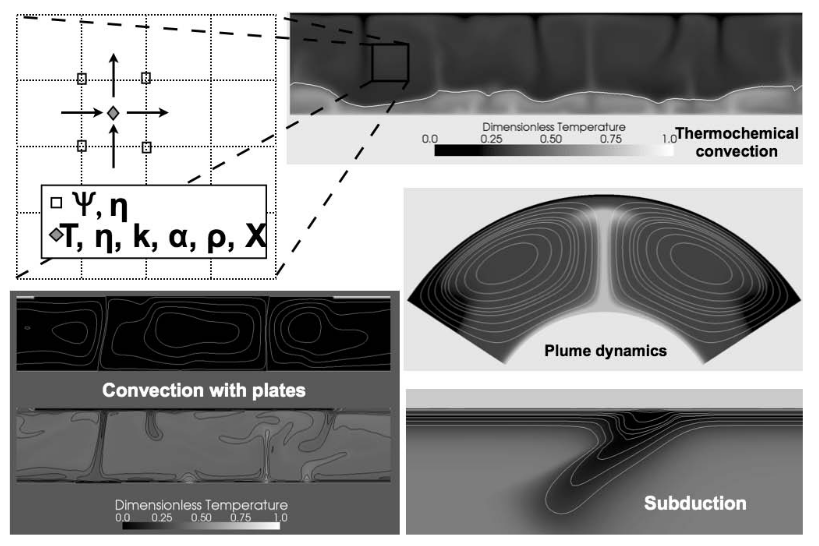
\includegraphics[width=13cm]{images/codes/streamV}

\begin{small}
\begin{itemize}
\item[2008]
\textcite{samu08} 
\item[2009]
\textcite{samu09} 
\item[2010]
\textcite{saev10}
\item[2011]
\textcite{saad11}
\item[2012]
\textcite{samu12b}
\item[2023]
\textcite{sasa23}
\end{itemize}
\end{small}

%------------------------------------------------------------------------------
\section{SubMar} 
%------------------------------------------------------------------------------

\begin{small}
\begin{itemize}
\item[\twothousandsix]       \textcite{masr06}
\item[\twothousandseven]     \textcite{masp07}
\item[\twothousandten]       \textcite{roms10}
\item[\twothousandtwelve]    \textcite{rosm12}
\item[\twothousandthirteen]  \textcite{rems13}
\item[\twothousandseventeen] \textcite{rerm17}
\item[\twothousandeighteen]  \textcite{marc18}
\item[\twothousandnineteen]  \textcite{rors19}
\item[\twothousandtwenty]    \textcite{rozr20}, \textcite{relr20}
\item[\twothousandtwentyone] \textcite{resr21}
\item[\twothousandtwentytwo] \textcite{bors22}
\end{itemize}
\end{small}

%------------------------------------------------------------------------------
\section{SULEC}
%------------------------------------------------------------------------------

\url{https://www.susannebuiter.eu/sulec.html}

\sulec is a 2D/3D arbitrary Lagrangian Eulerian finite-element 
code developed by Susanne Buiter and Susan Ellis. 
It solves the equation for conservation of momentum for an incompressible fluid combined with 
the heat equation. Pressure is calculated as mean stress following an Uzawa iterative penalty 
formulation (Pelletier \etal (1989) \cite{pefc89}). 
Materials are tracked with tracers which are advected with a 2nd-order Runge-Kutta scheme. 
A true free surface is obtained by a slight vertical stretch of the Eulerian mesh to 
accommodate surface displacements and the effects of surface processes (Fullsack \nineteenninetyfive \cite{full95}). 
\sulec includes a stabilization term that suppresses numerical overshoot of isostatic restoring forces 
at interfaces with strong density contrasts (Kaus \etal (\twothousandten) \cite{kamm10}; 
Quinquis \etal (\twothousandeleven) \cite{qube11}). The mechanical and thermal equations are solved using 
the direct sparse solver PARDISO (Schenk and Gaertner (twothousandfour) \cite{scga04}).

Not completely up to date (see website)
\begin{small}
\begin{itemize}
\item[\twothousandeleven]     \textcite{qube11}, \textcite{ellw11}
\item[\twothousandtwelve]     \textcite{buit12}, \textcite{tebu12},
                              \textcite{crsg12}, \textcite{grel12}
\item[\twothousandthirteen]   \textcite{ghbu13}
\item[\twothousandfourteen]   \textcite{ghbu14}, \textcite{qubu14}
\item[\twothousandfifteen]    \textcite{nabu15}
\item[\twothousandsixteen]    \textcite{zwsn16}, \textcite{elwr16}
\item[\twothousandseventeen]  \textcite{nabp17}
\item[\twothousandeighteen]   \textcite{tebu18}, \textcite{fade18},  \textcite{weef18}
\item[\twothousandnineteen]   \textcite{elgb19}, \textcite{biem19}
\item[\twothousandtwenty]     \textcite{pena20}
\item[\twothousandtwentytwo]  \textcite{pefb22} 
\item[\twothousandtwentyfour] \textcite{hube24} 
\end{itemize}
\end{small}




%%%%%%%%%%%%%%%%%%%%%%%%%%%%%%%%%%%%%%%%%%%%%%%%%%%%%%%%%%%%%%%%%%%%%%%%%%%%%%%
%TTTTTTTTTTTTTTTTTTTTTTTTTTTTTTTTTTTTTTTTTTTTTTTTTTTTTTTTTTTTTTTTTTTTTTTTTTTTTT
%%%%%%%%%%%%%%%%%%%%%%%%%%%%%%%%%%%%%%%%%%%%%%%%%%%%%%%%%%%%%%%%%%%%%%%%%%%%%%%

%------------------------------------------------------------------------------
\section{TDPOIS} 
%------------------------------------------------------------------------------

The numerics are explained in \cite{hous87} and the theory in \cite{hous90}.
This code is also called TDCON in \textcite{cosc06} (2006).

\begin{small}
\begin{itemize}
\item[\nineteeneightyseven]\textcite{hous87}
\item[\nineteenninety] \textcite{hous90} \textcite{hous90b}
\item[\nineteenninetyfive] \textcite{schh95} (check when I have access to pdf)
\item[\nineteenninetysix] \textcite{schh96}
\item[\twothousandtwo] \textcite{scbh02}
\item[\twothousandfour] \textcite{scbh04}
\item[\twothousandsix] \textcite{cosc06}
\end{itemize}
\end{small}




%------------------------------------------------------------------------------
\section{TERRA} 
%------------------------------------------------------------------------------
The computational grid is based on a projection of the regular icosahedron onto a 
sphere and successive dyadic refinements, see \textcite{bafr85}.  Concentric copies of such  
spherical layers of nodes build the domain in radial direction.
The first main improvement was being parallelised \textcite{buba95}.
Particles were added in \textcite{strb02}.

\begin{small}
\begin{itemize}
\item[\nineteeneightythree]    \textcite{baum83}
\item[\nineteeneightyfive]     \textcite{baum85}
\item[\nineteeneightyeight]    \textcite{glat88}
\item[\nineteenninetythree]    \textcite{tasg93}
\item[\nineteenninetyfour]     \textcite{tasg94}
\item[\nineteenninetyfive]     \textcite{buba95}
\item[\nineteenninetysix]      \textcite{buri96}
\item[\nineteenninetyseven]    \textcite{burb97},  \textcite{yang97}
\item[\nineteenninetyeight]    \textcite{burl98}
\item[\nineteenninetynine]     \textcite{tabg99},  \textcite{ribr99}, \textcite{resb99}
\item[\twothousandone]         \textcite{buda01},  \textcite{burm01}, \textcite{dabu01}
\item[\twothousandtwo]         \textcite{burb02},  \textcite{strb02}
\item[\twothousandthree]       \textcite{buht03},  \textcite{stjz03}
\item[\twothousandfour]        \textcite{resb04},  \textcite{wahb04}
\item[\twothousandfive]        \textcite{resb05},  \textcite{phbu05},  \textcite{funk05}
\item[\twothousandsix]         \textcite{dabu06},  \textcite{gowh06}
\item[\twothousandseven]       \textcite{phbu07},  \textcite{huda07b}
\item[\twothousandeight]       \textcite{heib08},  \textcite{shlj08},  \textcite{wahe08}
\item[\twothousandnine]        \textcite{phbs09},  \textcite{wodd09},
                               \textcite{gows09},  \textcite{iabu09},
                               \textcite{scbs09},  \textcite{scbs09b},
                               \textcite{scbr09},  \textcite{oebm09},
                               \textcite{dada09}
\item[\twothousandten]         \textcite{yayh10}
\item[\twothousandeleven]      \textcite{woda11},  \textcite{iahb11}
\item[\twothousandtwelve]      \textcite{dagd12},  \textcite{shbs12}
\item[\twothousandthirteen]    \textcite{dadb13},  \textcite{oflb13}, \textcite{wahe13}
\item[\twothousandfourteen]    \textcite{butm14}
\item[\twothousandfifteen]     \textcite{amsb15},  \textcite{cobs15}
\item[\twothousandsixteen]     \textcite{vade16},  \textcite{necg16}, \textcite{pric16}
\item[\twothousandseventeen]   \textcite{woda17},  \textcite{badw17}, \textcite{rubh17},
                               \textcite{wahe17} 
\item[\twothousandeighteen]    \textcite{ghbu18},  \textcite{cogb18}, \textcite{prda18}
\item[\twothousandnineteen]    \textcite{prdp19}
\item[\twothousandtwenty]      \textcite{cobo20}
\item[\twothousandtwentyone]   \textcite{ghbo21}
\item[\twothousandtwentytwo]   \textcite{licw22},  \textcite{brcb22}
\item[\twothousandtwentythree] \textcite{tabs23},  \textcite{padm23}
\end{itemize}
\end{small}


%------------------------------------------------------------------------------
\section{TERRA-NEO} 
%------------------------------------------------------------------------------

\begin{small}
\begin{itemize}
\item[\twothousandfifteen] \textcite{gmrs15}, \textcite{wegg15}
\item[\twothousandtwenty]  \textcite{babd20}
\end{itemize}
\end{small}

%------------------------------------------------------------------------------
\section{TerraFERMA} 
%------------------------------------------------------------------------------
TerraFERMA is the Transparent Finite Element Rapid Model Assembler, a software 
system for the rapid and reproducible construction and exploration of coupled multi-physics models.

TerraFERMA leverages three advanced open-source libraries for scientific computation that 
provide high level problem description (FEniCS), composable solvers for coupled multi-physics 
problems (PETSc) and a science neutral options handling system (SPuD) that allows the hierarchical 
management of all model options.

TerraFERMA inherits most of its functionality from the underlying libraries but adds a layer of 
control and guidance for building reusable and reproducible applications.

\url{http://terraferma.github.io/}

\begin{small}
\begin{itemize}
\item[\twothousandfourteen]  \textcite{wisv14}
\item[\twothousandsixteen]   \textcite{spmw16}
\item[\twothousandseventeen] \textcite{wisv17}, \textcite{ceww17}
\item[\twothousandnineteen]  \textcite{ceww19}, \textcite{perr19}
\item[\twothousandtwenty]    \textcite{siss20}, \textcite{abvw20}
\item[\twothousandtwentytwo] \textcite{ceap22}
\end{itemize}
\end{small}


%%%%%%%%%%%%%%%%%%%%%%%%%%%%%%%%%%%%%%%%%%%%%%%%%%%%%%%%%%%%%%%%%%%%%%%%%%%%%%%
%UUUUUUUUUUUUUUUUUUUUUUUUUUUUUUUUUUUUUUUUUUUUUUUUUUUUUUUUUUUUUUUUUUUUUUUUUUUUUU
%%%%%%%%%%%%%%%%%%%%%%%%%%%%%%%%%%%%%%%%%%%%%%%%%%%%%%%%%%%%%%%%%%%%%%%%%%%%%%%

%------------------------------------------------------------------------------
\section{UNDERWORLD 1\&2} 
%------------------------------------------------------------------------------
Section 3 of \cite{qums07} presents the evolutionary path which lead to this code.
Also check \cite{magm20} for Underworld2. 

\begin{center}
\includegraphics[width=5.5cm]{images/codes/underworld1}
\includegraphics[width=5.5cm]{images/codes/underworld2}
\includegraphics[width=5.5cm]{images/codes/underworld3}\\
{\captionfont Taken from a presentation by L. Moresi}
\end{center}


\begin{small}
\begin{itemize}
\item[\twothousandsix]       \textcite{stfs06},  \textcite{momu06}
\item[\twothousandseven]     \textcite{moql07},  \textcite{stfs07}, 
                             \textcite{qums07}
\item[\twothousandeight]     \textcite{lemm08},  \textcite{ozrs08}, 
                             \textcite{gotc08},  \textcite{stmt08},
                             \textcite{scsf11}
\item[\twothousandnine]      \textcite{stfm09} 
\item[\twothousandten]       \textcite{casm10},  \textcite{mamb10}, 
                             \textcite{stsf10},  \textcite{stfc10},
                             \textcite{fasm10},  \textcite{cazf10}
\item[\twothousandeleven]    \textcite{memm11},  \textcite{cafz11},  \textcite{leha11}
\item[\twothousandtwelve]    \textcite{cafa12},  \textcite{faca12}
\item[\twothousandthirteen]  \textcite{bemm12},  \textcite{scmo13}, 
                             \textcite{faca13},  \textcite{care13}, 
                             \textcite{coml13}
\item[\twothousandfourteen]  \textcite{famc14},  \textcite{shjm14},  \textcite{grbo14},
                             \textcite{comi14}
\item[\twothousandfifteen]   \textcite{quxm15},  \textcite{bemm15}, 
                             \textcite{scsp15},  \textcite{shmj15}, 
                             \textcite{carr15}
\item[\twothousandsixteen]   \textcite{shmv16},  \textcite{onlw16}, 
                             \textcite{kicf16},  \textcite{sacf16}
\item[\twothousandseventeen] \textcite{bems17},  \textcite{kicf17}, 
                             \textcite{sche17},  \textcite{wakc17}
\item[\twothousandeighteen]  \textcite{memm18},  \textcite{yamz18}, 
                             \textcite{bemc18},  \textcite{mord18},
                             \textcite{wakc18},  \textcite{wakc18b}
\item[\twothousandnineteen]  \textcite{samo19},  \textcite{yamg19}, 
                             \textcite{canc19},  \textcite{cakc19},
                             \textcite{sams19b}, \textcite{bore19},
                             \textcite{smbc19},  \textcite{canc19b}
\item[\twothousandtwenty]      \textcite{magm20},  \textcite{sams20},  \textcite{capi20}, 
                               \textcite{ghbm20},  \textcite{canc20},  \textcite{cofm20},
                               \textcite{gumc20},  \textcite{sche20}
\item[\twothousandtwentyone]   \textcite{kotr21},  \textcite{qizx21},
                               \textcite{stsc21},  \textcite{zhzl21},
                               \textcite{xiwk21},  \textcite{kncw21}
\item[\twothousandtwentytwo]   \textcite{wakw22},  \textcite{alrr22b}, \textcite{pefv22},
                               \textcite{olgr22},  \textcite{bahf22},  \textcite{canm22},
                               \textcite{wacw22},  \textcite{baha22},  \textcite{zugc22},
                               \textcite{aryt22}
\item[\twothousandtwentythree] \textcite{lass23}, \textcite{giln23}, \textcite{yaat23},
                               \textcite{scsb23}, \textcite{mord23}, \textcite{ligu23a},
                               \textcite{ligu23b}
\item[\twothousandtwentyfour]  \textcite{deyz24}, \textcite{gucm24}, \textcite{yuga24},
                               \textcite{comi24}

\end{itemize}
\end{small}


%%%%%%%%%%%%%%%%%%%%%%%%%%%%%%%%%%%%%%%%%%%%%%%%%%%%%%%%%%%%%%%%%%%%%%%%%%%%%%%
%VVVVVVVVVVVVVVVVVVVVVVVVVVVVVVVVVVVVVVVVVVVVVVVVVVVVVVVVVVVVVVVVVVVVVVVVVVVVVV
%%%%%%%%%%%%%%%%%%%%%%%%%%%%%%%%%%%%%%%%%%%%%%%%%%%%%%%%%%%%%%%%%%%%%%%%%%%%%%%

%------------------------------------------------------------------------------
\section{VEMAN}
%------------------------------------------------------------------------------

\begin{small}
\begin{itemize}
\item[2010] \textcite{bepo10}
\end{itemize}
\end{small}


%%%%%%%%%%%%%%%%%%%%%%%%%%%%%%%%%%%%%%%%%%%%%%%%%%%%%%%%%%%%%%%%%%%%%%%%%%%%%%%
%WWWWWWWWWWWWWWWWWWWWWWWWWWWWWWWWWWWWWWWWWWWWWWWWWWWWWWWWWWWWWWWWWWWWWWWWWWWWWW
%%%%%%%%%%%%%%%%%%%%%%%%%%%%%%%%%%%%%%%%%%%%%%%%%%%%%%%%%%%%%%%%%%%%%%%%%%%%%%%

%%%%%%%%%%%%%%%%%%%%%%%%%%%%%%%%%%%%%%%%%%%%%%%%%%%%%%%%%%%%%%%%%%%%%%%%%%%%%%%
%XXXXXXXXXXXXXXXXXXXXXXXXXXXXXXXXXXXXXXXXXXXXXXXXXXXXXXXXXXXXXXXXXXXXXXXXXXXXXX
%%%%%%%%%%%%%%%%%%%%%%%%%%%%%%%%%%%%%%%%%%%%%%%%%%%%%%%%%%%%%%%%%%%%%%%%%%%%%%%

%%%%%%%%%%%%%%%%%%%%%%%%%%%%%%%%%%%%%%%%%%%%%%%%%%%%%%%%%%%%%%%%%%%%%%%%%%%%%%%
%YYYYYYYYYYYYYYYYYYYYYYYYYYYYYYYYYYYYYYYYYYYYYYYYYYYYYYYYYYYYYYYYYYYYYYYYYYYYYY
%%%%%%%%%%%%%%%%%%%%%%%%%%%%%%%%%%%%%%%%%%%%%%%%%%%%%%%%%%%%%%%%%%%%%%%%%%%%%%%

%------------------------------------------------------------------------------
\section{YACC} 
%------------------------------------------------------------------------------
This stands for 'Yet Another Convection Code'.

\begin{small}
\begin{itemize}
\item[\twothousandten]       \textcite{toyc10}
\item[\twothousandeleven]    \textcite{yutc11}
\item[\twothousandtwelve]    \textcite{sato12}
\item[\twothousandthirteen]  \textcite{toyd13}
\item[\twothousandfifteen]   \textcite{tosn15}
\item[\twothousandsixteen]   \textcite{tomy16}
\end{itemize}
\end{small}

%%%%%%%%%%%%%%%%%%%%%%%%%%%%%%%%%%%%%%%%%%%%%%%%%%%%%%%%%%%%%%%%%%%%%%%%%%%%%%%
%ZZZZZZZZZZZZZZZZZZZZZZZZZZZZZZZZZZZZZZZZZZZZZZZZZZZZZZZZZZZZZZZZZZZZZZZZZZZZZZ
%%%%%%%%%%%%%%%%%%%%%%%%%%%%%%%%%%%%%%%%%%%%%%%%%%%%%%%%%%%%%%%%%%%%%%%%%%%%%%%

